 \chapter{Diseño del sistema mecatrónico }

 En este capítulo se desarrollará el diseño del sistema a partir del concepto óptimo de solución desarrollado en el capítulo anterior. Para comenzar, se presenta el sistema integrado en su totalidad y se describe su funcionamiento. Luego, se presentará el desarrollo del sistema electrónico. El cuál comprende la selección de componentes, los diagramas esquemáticos y el desarrollo de la placa electrónica. A continuación, se presentará el diseño mecánico. El cuál consiste de cálculos básicos, selección de componentes y materiales y descripción de planos de ensamble y despiece. Por último, se presentará el diseño del algoritmo de clasificación. El cuál incluye los diagramas de flujo que describen los algoritmos utilizados. Las hojas de datos y planos completos se pueden encontrar en los Anexos
 %******************* Aquí falta indicar que anexos*******************************

 \graphicspath{{Chapter4/Figuras/}{Chapter4/Figs/PDF/}{Chapter4/Figs/}{Chapter4/segundo/}}

\section{Integración del sistema mecatrónico}

\begin{figure}[htbp!]
\centering
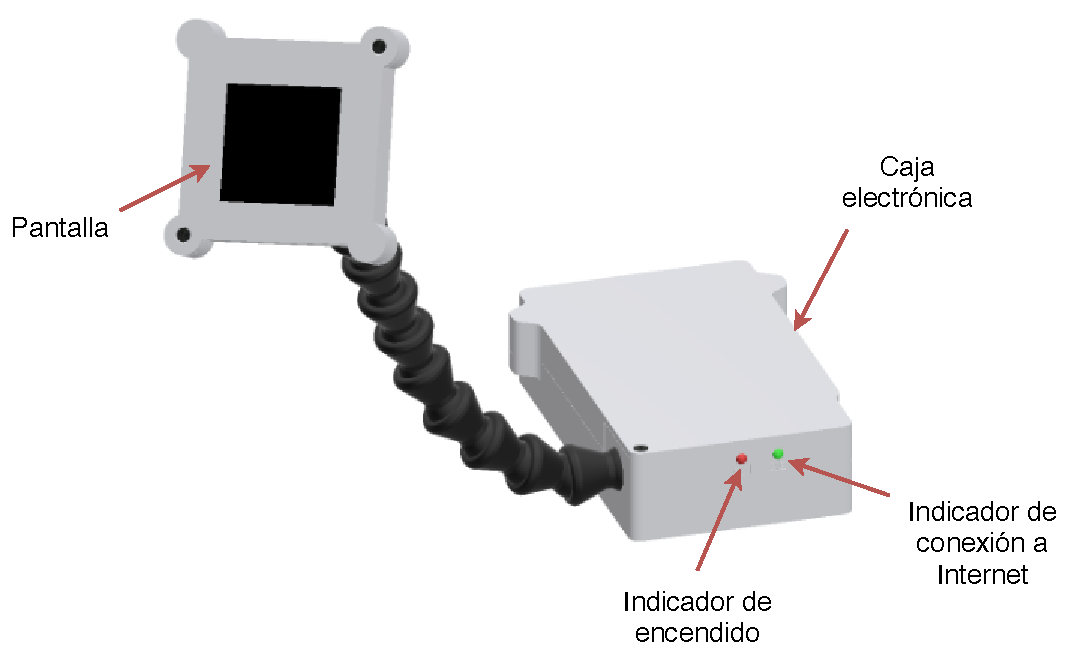
\includegraphics[width=\textwidth]{modelo_1.pdf}
\caption{Dispositivo de clasificación de estilo de conducción.}
\label{fig:modelo1}
\end{figure}

\begin{figure}[htbp!]
\centering
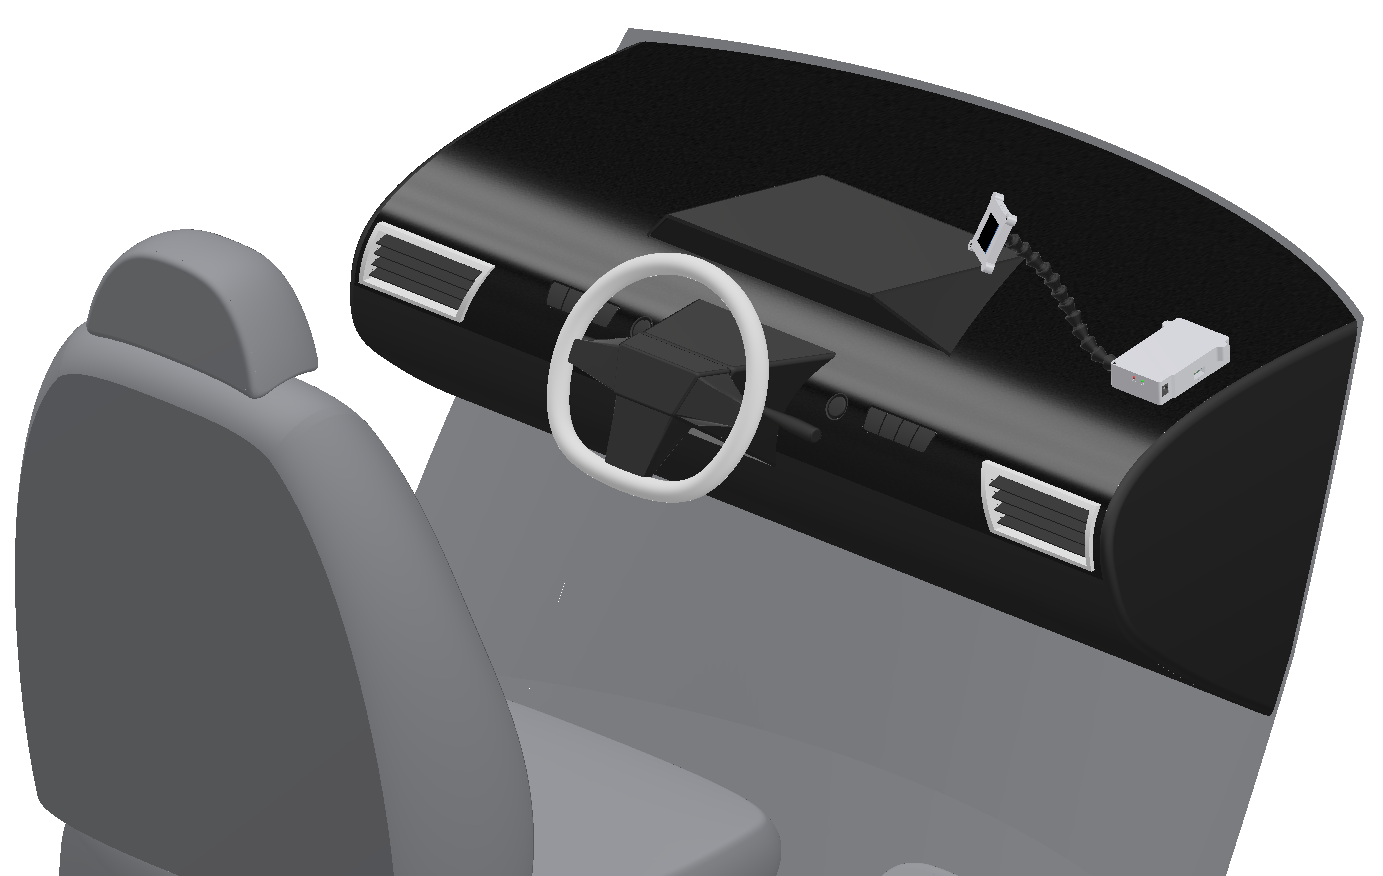
\includegraphics[width=\textwidth]{con_auto1.png}
\caption{Dispositivo de clasificación de estilo de conducción montado en un auto.}
\label{fig:modelo2}
\end{figure}

%Falta incluir otra figura de la vista superior con la tapa del case en transparencia
El sistema, Fig.~\ref{fig:modelo1} , esta compuesto por una placa electrónica que recogerá los datos de conducción usando sensores y estará contenida por una caja electrónica o case, se le llamará case principal. Estos datos se enviarán a través de la red 2G a un servidor y este responderá con el estilo de conducción, el cual se mostrará en la pantalla.

Este dispositivo estará colocado en el panel frontal del vehículo como se puede apreciar en la Fig.~\ref{fig:modelo2}. Para sujetar el dispositivo al panel se usa cinta adhesiva de doble contacto. El dispositivo cuenta con 4 puertos: Puerto de carga, ranura de tarjeta Nano SIM y 2 puertos SMA para las antenas de GPS y GPRS/GSM.


\section{Funcionamiento del sistema mecatrónico}
Para comenzar, se deben verificar la conexión de alimentación al dispositivo y su conexión a Internet antes de iniciar el viaje del vehículo. Esto se puede comprobar observando las luces indicadora de 'Encendido' y 'Conexión'. El dispositivo cuenta con una ranura para una tarjeta Nano SIM y solo se conectará a Internet si existe una de estas tarjetas insertada en el dispositivo que cuente con un plan de datos activo.

Luego de verificar que las conexiones funcionan, se inicia el viaje del vehículo. El conductor debe ajustar la posición de la pantalla de tal manera de que la pueda visualizar sin ningún problema y que no bloquee la vista de este. El sistema empezará a recolectar datos del IMU, del GPS y de los sensores internos del vehículo a través del módulo OBD2 desde que el sistema se conecta a Internet por primera vez. De esta manera se registra el inicio de un nuevo viaje. Los datos recolectados por los sensores se graban en el microcontrolador, quién obtendrá la ubicación , velocidad y aceleración exacta del vehículo al combinar los datos del IMU y del GPS. Además calculará el consumo de combustible de los datos obtenidos a través del módulo OBD2. Luego enviará estos datos a la nube, en donde se guardarán en una base de datos y se ejecutará el algoritmo de clasificación. Al clasificar los datos se envían de regreso al dispositivo, quién se encargará de mostrar el resultado de la clasificación al conductor por medio de la pantalla.

La pantalla mostrará tan solo un símbolo con un color representativo para evitar distracciones del conductor. De esta manera el conductor podrá conocer si se encuentra manejando de una manera agresiva o no, con tan solo una mirada a la pantalla. Cada maniobra clasificada con un  estilo de conducción del conductor es registrada durante todo el viaje en la nube y se le otorga un puntaje de acuerdo a su nivel de agresividad. Mientras menos agresiva sea su puntaje será mayor. Se calculará luego un puntaje para toda la trayectoria realizada al sumar los puntajes de cada maniobra. Al final del día el conductor habrá realizado varias trayectorias y se calculará un promedio que se le asignará como indicador de desempeño.



\section{Diseño electrónico}
En esta sección se presentará primero el diagrama de bloques general del dispositivo. Luego se desarrollará la selección de cada componente y el diseño de las conexiones y de la placa electrónica.

\subsection{Diagrama de bloques}
En la Fig.~\ref{fig:bloques} se tiene el diagrama de bloques del dispositivo. El pre-procesamiento y la recolección de los datos de los sensores se llevará a cabo por medio de un ESP-WROOM-32. A este están conectados un IMU de 6 ejes (ICM-20648), por medio del protocolo I\textsuperscript{2}C; un módulo GPS (NEO-M8N), por medio de comunicación serial y una pantalla de tecnología IPS LCD (Con el controlador ST7789), por medio del protocolo SPI. El ESP-WROOM-32 enviará los datos pre-procesados por medio de un módulo GPRS/GSM (SIM800L), que se encuentra conectado a él por medio de comunicación serial. Por último el módulo OBD2 se encuentra conectado al puerto OBD2 del vehículo y se comunica inalámbricamente con el ESP-WROOM-32 usando comunicación serial a través de Bluetooth.

Todos estos elementos se alimentan usando la energía disponible del vehículo (\SI{12}{V} de la batería). El módulo OBD2 es el único elemento que se encuentra se parado del dispositivo principal y obtiene su energía a través del mismo puerto OBD2 por el cual esta conectado al vehículo. LOs demás componentes no pueden ser alimentados directamente con \SI{12}{V}, por lo que se necesita transformar el voltaje de acuerdo a los requerimientos de cada elemento. Esto se realiza en dos etapas, ya que se necesitan solo 2 voltajes distintos: \SI{4}{V} y \SI{3.3}{V}. La primera etapa de reducción se lleva a cabo por un regulador switching (TPS563210) que se encarga de regular el voltaje de \SI{12}{V} a \SI{4}{V} para alimentar al módulo GPRS/GSM (SIM800L). Luego se usa un regulador LDO (LT1764A) que se encarga de regular el voltaje de \SI{4}{V} a \SI{3.3}{V} que servirán para alimentar al microcontrolador, módulo GPS, IMU y a la pantalla.


\begin{figure}[htbp!]
\centering
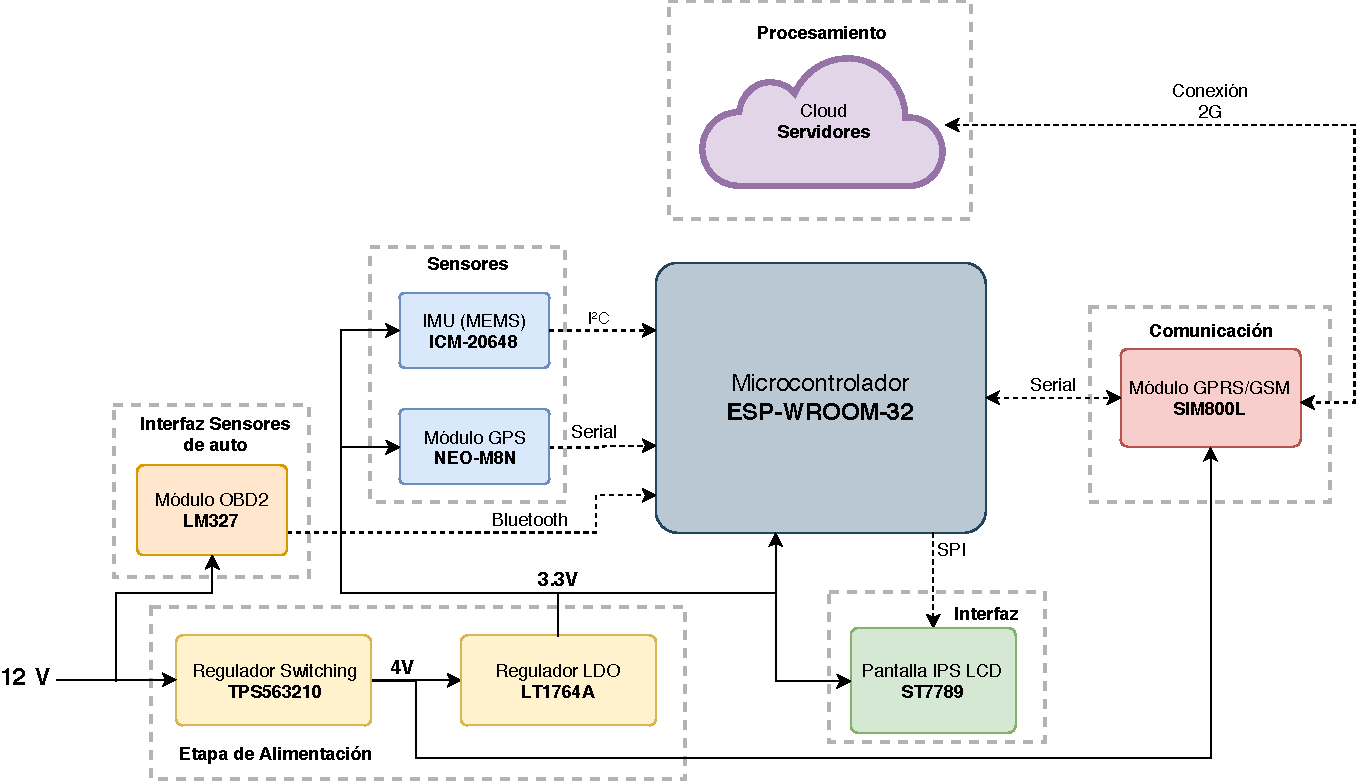
\includegraphics[width=\textwidth]{Bloques_principal.pdf}
\caption{Diagrama de bloques.}
\label{fig:bloques}
\end{figure}

\subsection{Componentes electrónicos}


\subsubsection{Inertial Measurement Unit (IMU)}
Este dispositivo cuenta con un acelerómetro, un giroscopio. Los datos registrados por estos sensores se pueden combinar para obtener el perfil de velocidad y aceleración, tanto longitudinal como lateral, del vehículo y estos perfiles aportan mucha información acerca del estilo de conducción del usuario.

Para seleccionar este componente empecemos por determinar las características que este debe poseer. En primer lugar el rango de medición debe ser el adecuado. En las investigaciones citadas  \cite{6957822}, \cite{constantinescu}, \cite{6083078},  \cite{Va-2013} La aceleración de los vehículos se suele encontrar dentro del rango de \SI{\pm7}{m/s^2}. Los rangos de medición de los acelerómetros se suelen expresar en \SI{}{g}, así que se necesita un acelerómetro que pueda medir en un rango de por lo menos \SI{\pm0.7}{g}

Realizando el mismo análisis para el giroscopio, en \cite{6083078} y \cite{6629603} se tiene que el rango mínimo de medición es de \SI{\pm57}{rad/s}

\bgroup
\def\arraystretch{1.5}%  1 is the default, change whatever you need
\begin{table}[htbp!]
\centering
\caption[Sensibilidad y Rango del ICM-20648]{Sensibilidad y Rango del ICM-20648 \cite{ICM20648}.}
\begin{tabular}{@{}P{3cm}P{3cm}P{3cm}P{3cm}@{}}
\toprule
Rango del Giroscopio (\si{\degree/sec}) & Sensibilidad del Giroscopio (\si{LSB/\degree/sec}) & Rango del Acelerómetro     (\si{g}) & Sensibilidad del Acelerómetro (\si{LSB/g}) \\ \midrule
\num{\pm 250} & 131 & \num{\pm 2} & 16384 \\
\num{\pm 500} & 65.5 & \num{\pm 4} & 8192 \\
\num{\pm 1000} & 32.8 & \num{\pm 8} & 4096 \\
\num{\pm 2000} & 16.4 & \num{\pm 16} & 2048 \\ \bottomrule
\end{tabular}
\label{diag:IMU1}
\end{table}

\egroup

El sensor que se eligió debido a que cumple con las características mencionadas anteriormente es el \textbf{ICM-20648} (Fig.~\ref{fig:IMU}) producido por TDK InvenSense. En las Tablas \ref{diag:IMU1} y \ref{diag:IMU2} se muestran sus principales características.


\bgroup
\def\arraystretch{1.5}%  1 is the default, change whatever you need
\begin{table}[htbp!]
\centering
\caption[Condiciones de Operación del ICM-20648]{Condiciones de Operación del ICM-20648 \cite{ICM20648}.}
\begin{tabular}{@{}ll@{}}
\toprule
Características & Valor \\ \midrule
Voltaje de alimentación & \SI{1.71}{V} - \SI{3.6}{V} \\
Corriente de operación & \SI{3.2}{mA} \\
Temperatura de operación & \SI{-40}{\celsius} hasta \SI{85}{\celsius} \\
Salida digital & I\textsuperscript{2}C o SPI \\
DMP & Onboard Digital Motion Processor \\ \bottomrule
\end{tabular}
\label{diag:IMU2}
\end{table}

\egroup

\begin{figure}[htb!]
\centering
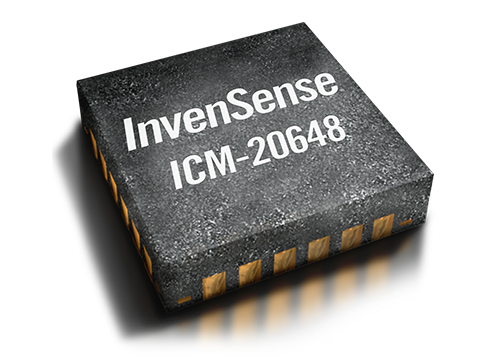
\includegraphics[width=0.4\textwidth]{ICM-20648.png}
\caption{ICM-20648, IMU de 6 grados de libertad.}
\label{fig:IMU}
\end{figure}

\newpage

\subsubsection{Módulo GPS}
Este módulo se encargará de detectar la posición exacta del vehículo en coordenadas. Para hacer esto se puede recurrir a distintos servicios del Sistema mundial de navegación por satélite (GNSS). Actualmente se encuentran dos operativos completamente: GPS y GLONASS. Es primero es el servicio hecho por Estados Unidos y el segundo es el realizado por Rusia. Es importante considerar la capacidad de los diferentes módulos para poder acceder a estos dos servicios.

Las características que debe tener el módulo de GPS son las siguientes:
\begin{itemize}
    \itemsep0em
    \item Bajo consumo.
    \item Poder acceder tanto a GPS como a GLONASS.
    \item Por lo menos una frecuencia de muestreo de \SI{1}{Hz}.
\end{itemize}

El modulo de GPS que cumple con estas características es el \textbf{NEO-M8N} de Ublox (Fig.~\ref{fig:GPS}). En la Tabla~\ref{diag:GPS} se resumen sus principales características.
\begin{figure}[hbtp!]
\centering
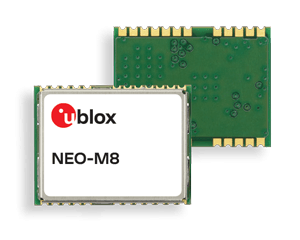
\includegraphics[width=0.5\textwidth]{NEO-M8.png}
\caption[NEO-M8N, módulo GPS]{NEO-M8N, módulo GPS \cite{GPS}.}
\label{fig:GPS}
\end{figure}

\bgroup
\def\arraystretch{1.5}%  1 is the default, change whatever you need
\begin{table}[htbp!]
\centering
\caption[Características del NEO-M8N]{Características del NEO-M8N \cite{GPS}.}
\begin{tabular}{@{}ll@{}}
\toprule
Características & Valor \\ \midrule
GNSS & GPS, GLONASS, GALIEO y BeiDou \\
Precisión & \SI{2.5}{m} \\
Frecuencia máxima & \SI{5}{Hz} \\
Protocolos de Comunicación & UART, I\textsuperscript{2}C, SPI \\
Voltaje de operación & \SI{2.7}{V} - \SI{3.6}{V} \\
Corriente de operación & \SI{32}{mA} \\
Corriente máxima & \SI{67}{mA} \\
Temperatura de Operación & \SI{-40}{\celsius} hasta \SI{85}{\celsius} \\\bottomrule
\end{tabular}
\label{diag:GPS}
\end{table}
\egroup






\subsubsection{Módulo GPRS/GSM}
El módulo GPRS/GSM es capaz de conectarse a las red 2G. Esta red es la que tiene mayor cobertura en el Perú (Fig.~\ref{fig:Cobertura}) ya que es la más antigua. Esta red puede alcanzar hasta una velocidad de \SI{114}{kbps} y es la de menor consumo energético, comparada con 3G y 4G. Usando este módulo se enviarán los datos recopilados por el sistema a través de Internet y se asegurará su conexión en todo momento.

\begin{figure}[hbtp!]
\centering
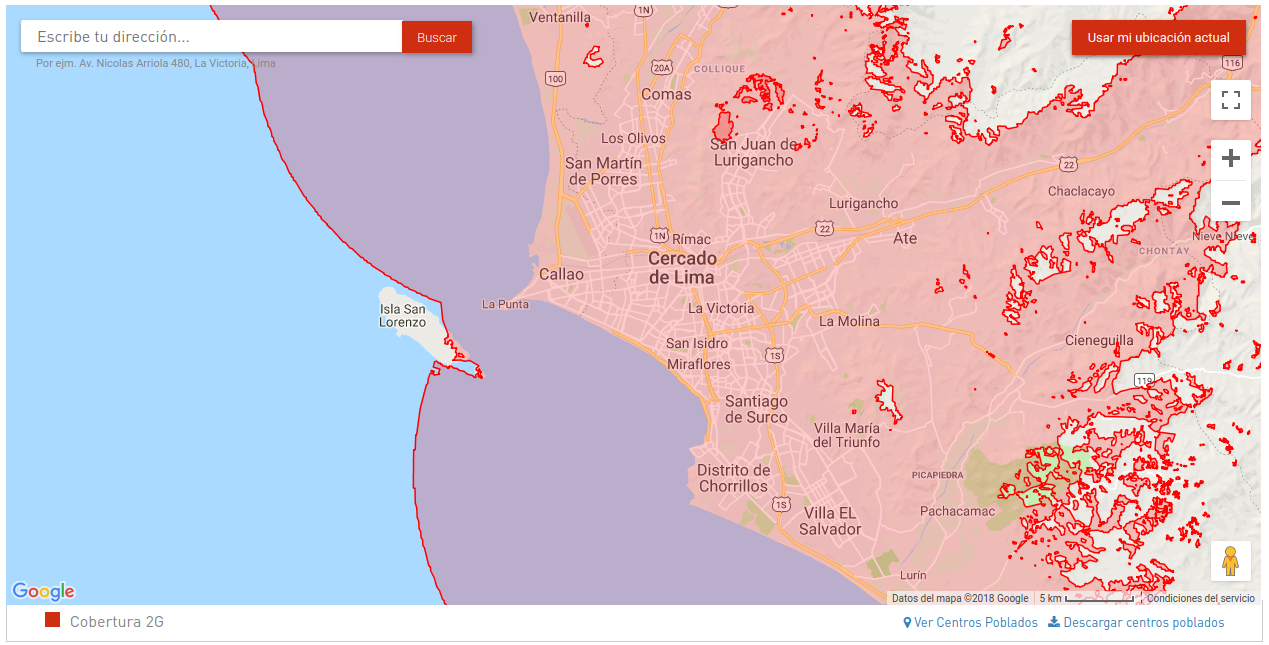
\includegraphics[width=\textwidth]{Cobertura_2G.png}
\caption[Cobertura de la red 2G de Claro]{Cobertura de la red 2G de Claro \cite{Cobertura_claro}.}
\label{fig:Cobertura}
\end{figure}

Una opción muy popular es el módulo \textbf{SIM 800L} (Fig.~\ref{fig:SIM}) que debido a sus características, expuestas en la Tabla~\ref{diag:SIM}, su disponibilidad y su bajo precio lo hacen adecuado para ser usado en este sistema.

\begin{figure}[hbtp!]
\centering
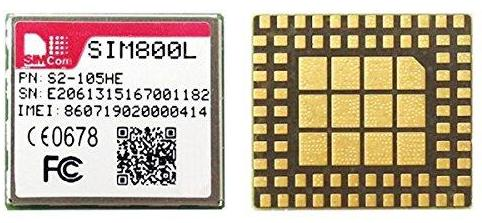
\includegraphics[width=0.6\textwidth]{SIM800L.jpg}
\caption[SIM 800L, módulo GPRS/GSM]{SIM 800L, módulo GPRS/GSM \cite{SIM800L}.}
\label{fig:SIM}
\end{figure}

\bgroup
\def\arraystretch{1.5}%  1 is the default, change whatever you need
\begin{table}[htbp!]
\centering
\caption[Características del SIM 800L]{Características del SIM 800L \cite{SIM800L}.}
\begin{tabular}{@{}p{5.4cm}p{8cm}@{}}
\toprule
Características & Valor \\ \midrule
Voltaje de operación & \SI{3.4}{V} -  \SI{4.4}{V} \\
Corriente promedio en Reposo & \SI{18.7}{mA} \\
Corriente promedio durante \mbox{transmisión} & \SI{453.57}{mA} \\
Corriente máxima & \SI{2}{A} (Solo durante ráfaga de transmisión) \\
Temperatura de operación & \SI{-40}{\celsius} hasta \SI{85}{\celsius} \\
Velocidad de transmisión & máx. \SI{85.6}{kbps} \\
Bandas de frecuancia & Quad-band: GSM 850, EGSM 900, DCS 1800, PCS 1900 \\ \bottomrule
\end{tabular}
\label{diag:SIM}
\end{table}
\egroup






\subsubsection{Pantalla}
La pantalla cumplirá el rol de mostrar la clasificación del estilo de conducción del usuario. Para poder transmitir la información sin generar distracciones se usarán símbolos y colores para representar los estilos de conducción.

Además se necesita que la pantalla se pueda observar bien tanto a la luz del día, por lo que su ángulo de visibilidad y su brillo serán factores importantes también.

Por último, el tamaño de la pantalla debe permitir la identificación del símbolo por parte del conductor. Basados en estos parámetros se puede elegir entre usar 3 tecnologías muy populares: LCD, OLED e IPS LCD.

Las pantallas LCD pueden alcanzar una densidad de imagen más alta que las OLED. Sin embargo, las OLED tienen un mejor ángulo de visión y un menor consumo. Por otro lado, las IPS LCD tienen también un muy buen ángulo de visión y buena densidad de imagen.

\bgroup
\def\arraystretch{1.5}%  1 is the default, change whatever you need
\begin{table}[htb!]
\centering
\caption{Alternativas de pantallas}
\begin{tabular}{@{}p{1.6cm}lllP{3cm}lc@{}}
\toprule
Nr. \mbox{Producto} & Tecnología & Controlador & Tamaño & Voltaje de Operación & Precio & Resolución\\ \midrule
1431 & OLED & SSD1351 & \SI{1.5}{in} & \SI{3.3}{V} o \SI{5}{V} & \textdollar \num{39.95} & 128x128\\
2088 & LCD & ST7735R & \SI{1.44}{in} & \SI{3.3}{V} o \SI{5}{V} & \textdollar \num{14.95} & 128x128\\
3787 & IPS LCD & ST7789 & \SI{1.54}{in} & \SI{3.3}{V} o \SI{5}{V} & \textdollar \num{19.95} & 240x240\\ \bottomrule
\end{tabular}
\label{diag:Display}
\end{table}
\egroup

En la Tabla.~\ref{diag:Display} se pueden ver 3 alternativas para la pantalla. De estas se escoge la pantalla IPS LCD (Fig.~\ref{fig:Display}), ya que tiene buen ángulo de visibilidad, tamaño y resolución.


\begin{figure}[hbt!]
\centering
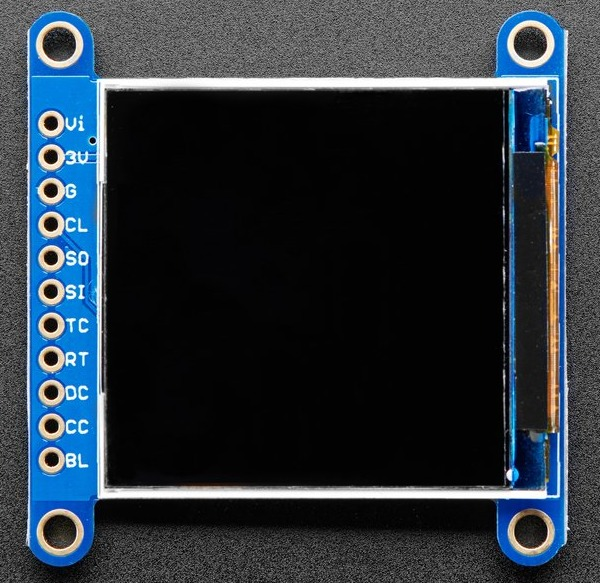
\includegraphics[width=0.5\textwidth]{IPS_LCD.jpg}
\caption[Adafruit 1.54" 240x240 Wide Angle TFT LCD Display - ST7789]{Adafruit 1.54" 240x240 Wide Angle TFT LCD Display - ST7789 \cite{IPS_LCD}.}
\label{fig:Display}
\end{figure}


\newpage








\subsubsection{Módulo OBD2}
Este módulo se encargará de acceder a todos los parámetros internos del auto conectándose directamente a las ECU \textit{(Electronic Control Units)} del motor. Para poder leer estos parámetros diversas marcas de autos usan distintos protocolos de comunicación. En la Tabla~\ref{diag:OBD} Se muestran distintos protocolos y en cada columna circuitos integrados ELMXXX que se usan para comunicarse con el puerto OBD2.

\bgroup
\def\arraystretch{1.5}%  1 is the default, change whatever you need
\begin{table}[htbp!]
\centering
\caption[Protocolos y Circuitos integrados]{Protocolos y Circuitos integrados \cite{OBD}.}
\begin{tabular}{|l|P{1.5cm}|P{1.5cm}|P{1.5cm}|P{1.5cm}|P{1.8cm}|}
\hline
 &  ELM323 & ELM325 & ELM327  & ELM329 & ELM329L \\ \hline
SAE J1850-PWM   &  &  & \si{\surd}  &  &  \\ \hline
SAE J1850-VPW   &  &  & \si{\surd}  &  &  \\ \hline
ISO 9141-2   & \si{\surd} &  & \si{\surd}  &  &  \\ \hline
ISO 14230-4 (slow)     & \si{\surd} &  & \si{\surd}  &  &  \\ \hline
ISO 14230-4 (fast)     & \si{\surd} &  & \si{\surd} &  \si{\surd} & \si{\surd} \\ \hline
ISO 15765-4 (CAN)     &  &  & \si{\surd} & \si{\surd} &  \si{\surd} \\ \hline
SAE J1939 (250kbps)     &  &  & \si{\surd} & \si{\surd} &  \si{\surd} \\ \hline
SAE J1939 (500kbps)     &  &  & \si{\surd} & \si{\surd} & \si{\surd} \\ \hline
SAE J1708 (J1587)     &  & \si{\surd} &  &    &  \\ \hline
SAE J1708 (J1922)     &  & \si{\surd} &  &    &  \\ \hline
\end{tabular}
\label{diag:OBD}
\end{table}
\egroup

Para maximizar la compatibilidad con vehículos se escoge el modulo \textbf{ELM327}. Este IC convierte los protocolos mencionados a comunicación serial y puede transmitir los datos a través de un cable, WiFi o Bluetooth. Para esta aplicación se escoge la versión que usa Bluetooth (Fig.~\ref{fig:OBD}) ya que el conector se encontrará a menos de \SI{2}{m} del conector, permitiéndole usar esta tecnología que consume menos energía que el WiFi y es inalámbrica también.

\begin{figure}[hbtp!]
\centering
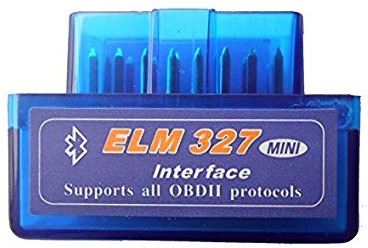
\includegraphics[width=0.5\textwidth]{OBD.jpg}
\caption[ELM327 - OBD2 interface]{ELM327 - OBD2 interface \cite{OBD}.}
\label{fig:OBD}
\end{figure}








\subsubsection{Microcontrolador}
El microcontrolador a seleccionar necesita poder comunicarse con todos los módulos anteriores, poder manejar protocolos como MQTT y CoAP y además realizar procesamiento básico de fusión de sensores (mezclar los datos obtenidos del IMU y del GPS). Se ha escogido para este sistema al ESP-WROOM-32 (Fig.~\ref{fig:esp-wroom32})

Este microcontrolador cuenta con el diagrama de bloques expuesto en la Fig.~\ref{fig:Bloques_esp32} y como se puede apreciar, cuenta con I\textsuperscript{2}C para comunicarse con el IMU, UART para comunicarse con el módulo GPS y el módulo GPRS/GSM, SPI para controlar la pantalla y Bluetooth para comunicarse con el módulo OBD2. Además presenta la suficiente potencia para realizar las tareas anteriormente descritas. Un resumen de sus características se encuentra en la Tabla~\ref{diag:ESP32}.

\begin{figure}[hbtp!]
\centering
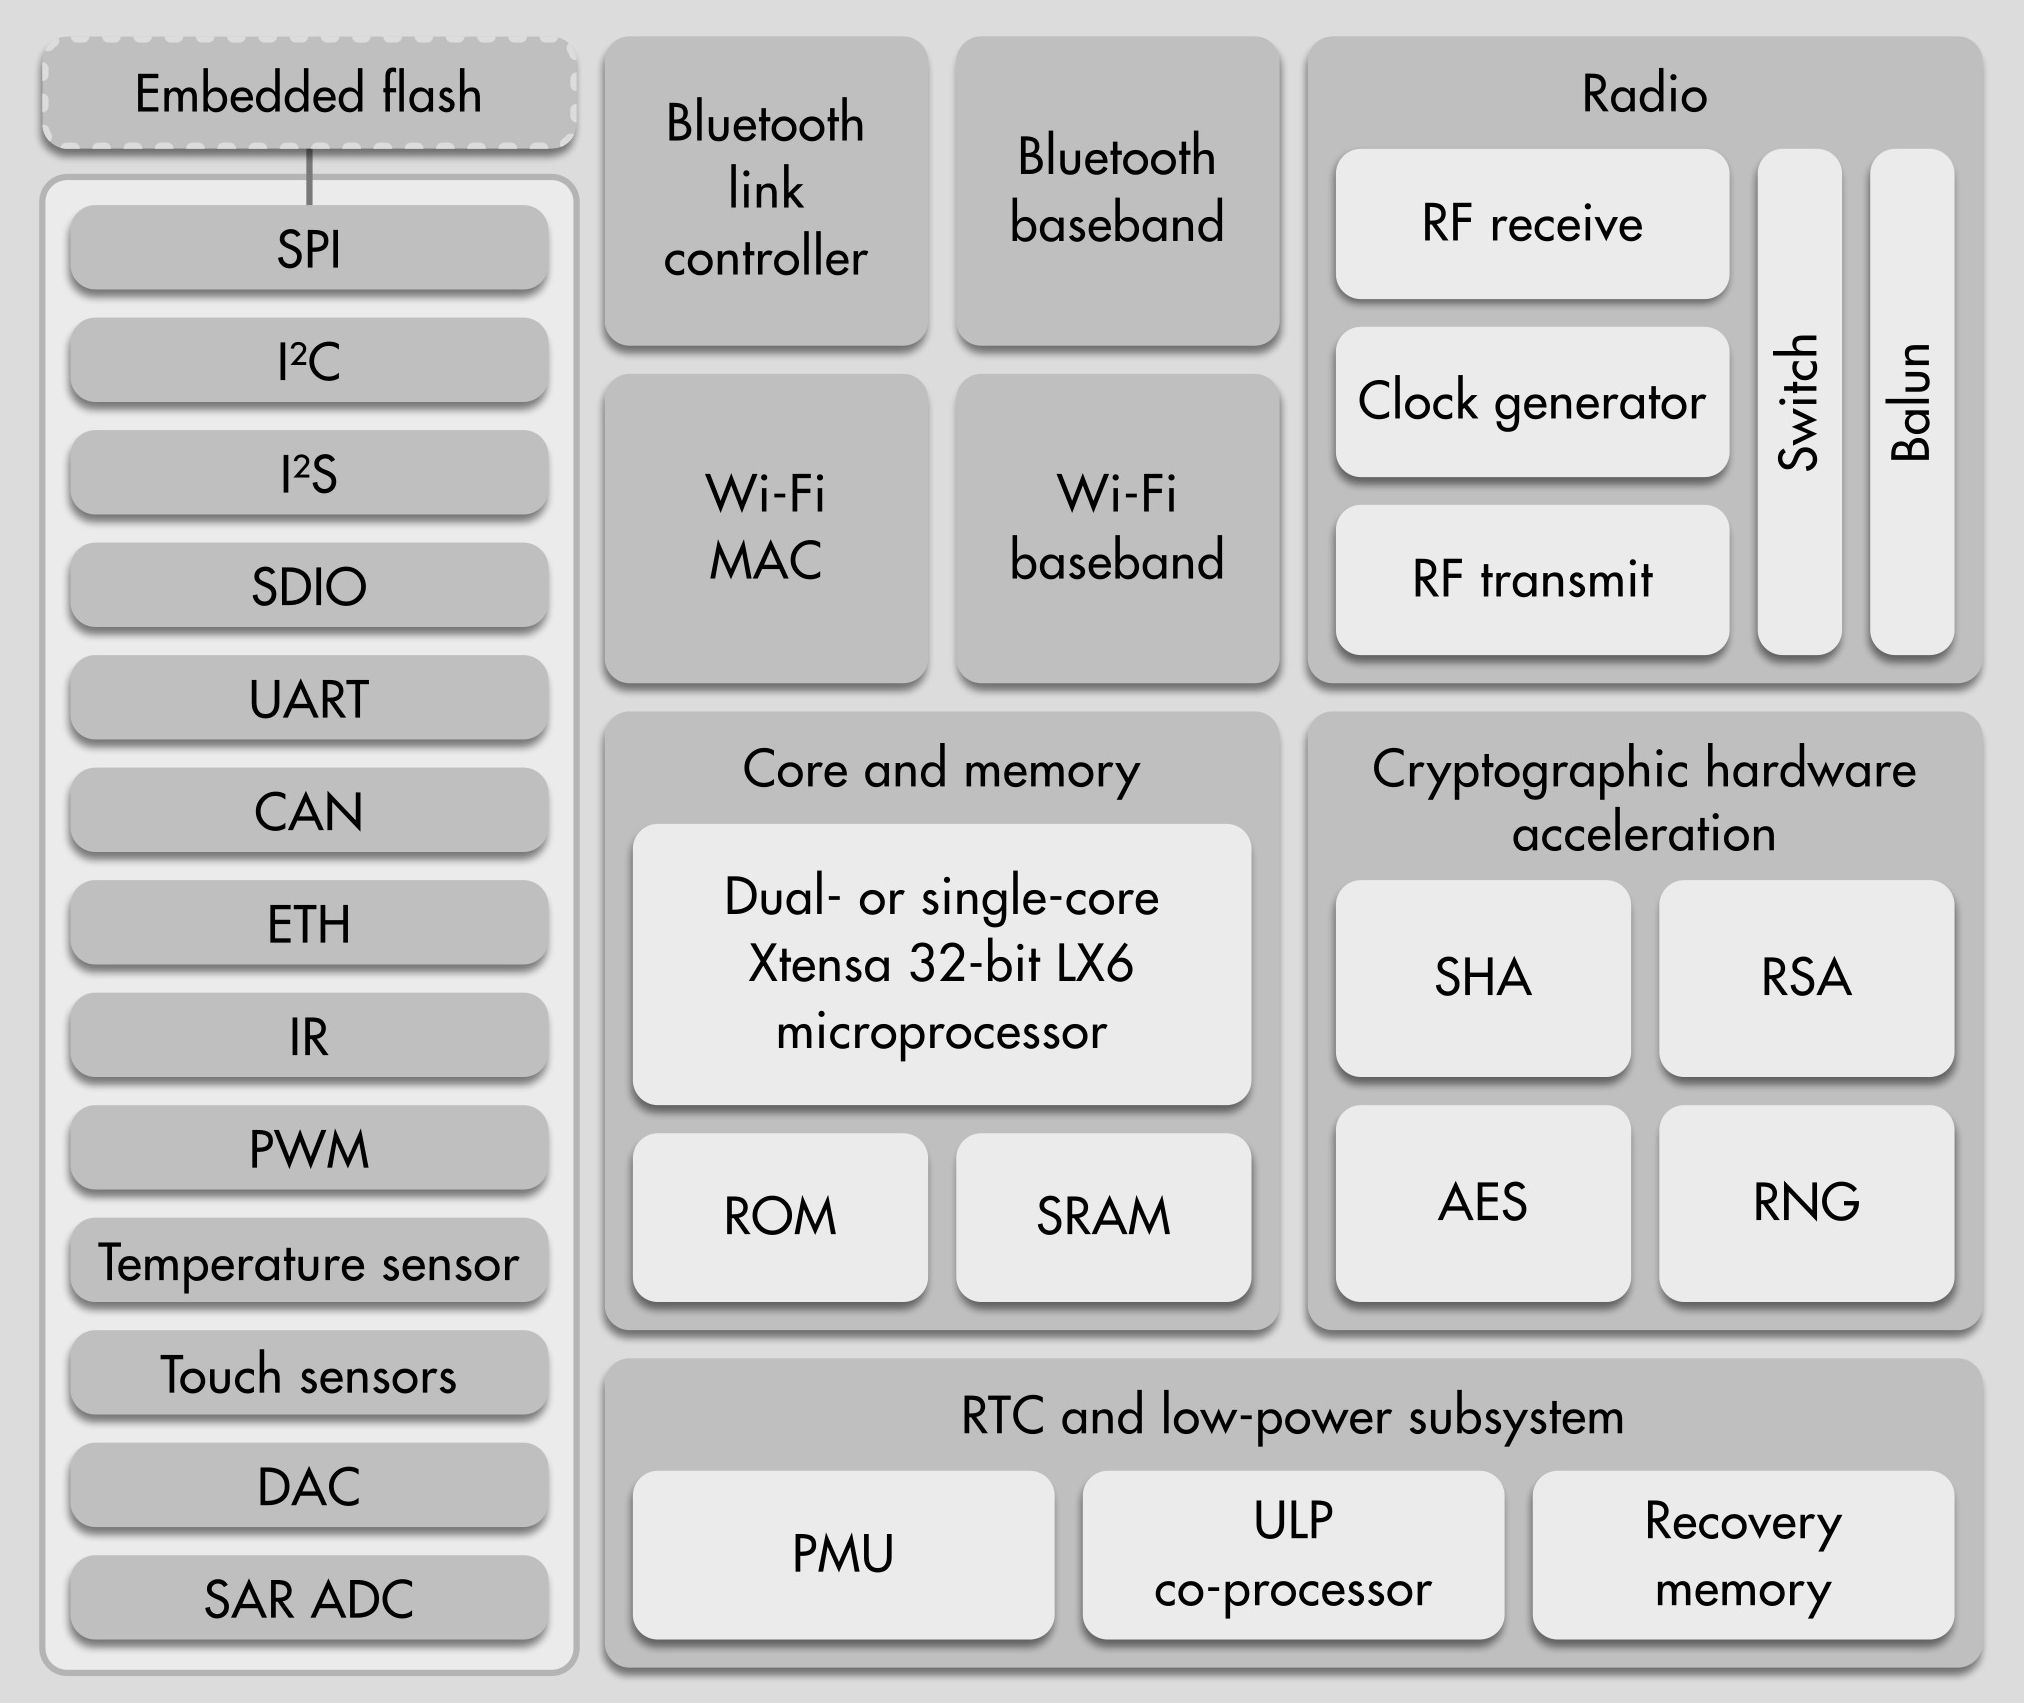
\includegraphics[width=0.9\textwidth]{ESP32_Function_Block_Diagram.jpg}
\caption{Diagrama de Bloques del ESP32  \cite{Esp32}.}
\label{fig:Bloques_esp32}
\end{figure}


\begin{figure}[hbtp!]
\centering
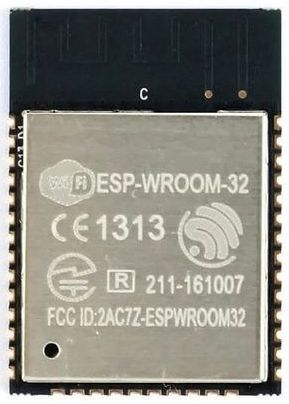
\includegraphics[width=0.3\textwidth]{esp32.jpg}
\caption{ESP-WROOM-32 \cite{ESP32_page}.}
\label{fig:esp-wroom32}
\end{figure}

\bgroup
\def\arraystretch{1.5}%  1 is the default, change whatever you need
\begin{table}[htbp!]
\centering
\caption[Características del ESP-WROOM-32]{Características del ESP-WROOM-32 \cite{Esp32_Hardware}.}
\begin{tabular}{@{}lp{9cm}@{}}
\toprule
Características & Valor \\ \midrule
Voltaje de Operación & \SI{2.7}{V} - \SI{3.6}{V} \\
Corriente máxima & \SI{500}{mA} \\
Corriente de operación & \SI{80}{mA} \\
Corriente en sleep mode & \SI{5}{\uA} \\
Frecuencia del CPU & \SI{240}{MHz} \\
Temperatura de operación & \SI{-40}{\celsius} hasta \SI{85}{\celsius} \\
Interfaces & SD card, UART, SPI, SDIO, I\textsuperscript{2}C, LED PWM, Motor PWM, I 2 S,IR, contador de pulsos, GPIO, sensor táctil capacitivo, ADC, DAC \\
Connectividad & WiFi (802.11 b/g/n (802.11n up to 150 Mbps) Bluetooth (Bluetooth v4.2 BR/EDR y BLE)\\\bottomrule
\end{tabular}
\label{diag:ESP32}
\end{table}
\egroup









\subsubsection{Regulador switching}
Una vez escogidos los componentes a usar en las secciones anteriores, se calculará el consumo total de los componentes para poder diseñar la etapa de alimentación del sistema. En la Tabla~\ref{diag:consumo} se encuentra un resumen de cada dispositivo con su voltaje de operación y su corriente máxima de consumo.

\bgroup
\def\arraystretch{1.5}%  1 is the default, change whatever you need
\begin{table}[htbp!]
\centering
\caption[Consumo de los componentes del sistema]{Consumo de los componentes del sistema.}
\begin{tabular}{@{}lp{2cm}p{2cm}p{2cm}@{}}
\toprule
Dispositivo & Voltaje de Operación & Corriente máxima & Potencia máxima\\ \midrule
IMU (ICM-20648) & \SI{3.3}{V} & \SI{3.2}{\mA} & \SI{10.56}{\mW} \\
Módulo GPS (NEO-M8N) & \SI{3.3}{V} & \SI{67}{mA} & \SI{221,1}{\mW}\\
Módulo GPRS/GSM (SIM800L) & \SI{4}{V} & \SI{2000}{mA} & \SI{8000}{\mW}\\
Pantalla IPS LCD & \SI{3.3}{V} & \SI{50}{mA} & \SI{165}{\mW}\\
OBD2 (ELM237) & \SI{5}{V} & \SI{12}{mA} & \SI{60}{\mW}\\
ESP-WROOM-32 & \SI{3.3}{V} & \SI{500}{mA} & \SI{1650}{\mW}\\ \bottomrule
\end{tabular}
\label{diag:consumo}
\end{table}
\egroup

Sin embargo, El módulo OBD2 (ELM237) no estará conectado junto con los demás componentes. Este módulo se conectará al puerto OBD2 del Auto y obtendrá energía de esta misma conexión sin necesidad de diseñarle un regulador de voltaje.


Si sumamos la potencia máxima de cada dispositivo, obtendremos la potencia mínima necesaria que se debe poder entregar por el regulador de voltaje. Esta suma da como resultado \textbf{10.046 W}.


\begin{figure}[hbtp!]
\centering
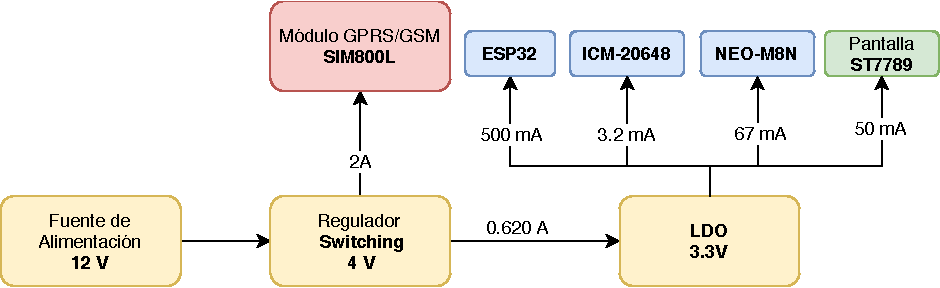
\includegraphics[width=\textwidth]{Bloques_Alimentacion.pdf}
\captionsetup{justification=centering,margin=2cm}
\caption{Diagrama de bloques de las etapas de alimentación con la corriente máxima de cada dispositivo.}
\label{fig:bloques_alim}
\end{figure}



Se propone dos etapas de regulación de voltaje debido a que se necesitan 2 niveles de voltaje, \SI{4}{V} y \SI{3.3}{V}. En la primera etapa se usará un regulador switching para obtener \SI{4}{V} de los \SI{12}{V} disponibles en la alimentación. Y en la segunda etapa se usará un LDO (Low Dropout Regulator) para obtener los \SI{3.3}{V} a partir de los \SI{4}{V}. En la Fig.~\ref{fig:bloques_alim} se dispone de manera gráfica e ideal la potencia y las corrientes máximas que deben poder entregar los reguladores de voltaje.



Entonces usando  la Fig.~\ref{fig:bloques_alim} Se tiene que el regulador switching debe poder entregar por lo menos \SI{2.62}{A}. Se selecciona el circuito integrado \textbf{TPS563210} que tiene las características mencionadas en la Tabla~\ref{diag:Switching}

\bgroup
\def\arraystretch{1.5}%  1 is the default, change whatever you need
\begin{table}[htbp!]
\centering
\caption[Características del TPS563210]{Características del TPS563210 \cite{TPS563210}.}
\begin{tabular}{@{}ll@{}}
\toprule
Características & Valor \\ \midrule
Voltaje de entrada & \SI{4.5}{V} - \SI{17}{V} \\
Voltaje de salida & \SI{0.76}{V} - \SI{7}{V} \\
Corriente máxima de operación & \SI{3}{A} \\
Frecuencia de conmutación & \SI{650}{kHz} \\
Temperatura de operación de la juntura & \SI{-40}{\celsius} - \SI{150}{\celsius}\\
Resitencia térmica de juntura-ambiente & \SI{87}{\celsius/W}\\\bottomrule
\end{tabular}
\label{diag:Switching}
\end{table}
\egroup


Se calcula entonces si este regulador switching es capaz de entregar \SI{2.62}{A} o \SI{10.046}{W} sin usar un disipador. Para esto se usa la Ecuación~\ref{eq:disipadores}
\begin{equation}
   T_J=T_A+(R_{\theta JA} \times Potencia_{dis})
   \label{eq:disipadores}
\end{equation}

La $Potencia_{dis}$ en esta ecuación es la potencia disipada la cual se puede calcular a partir de la eficiencia del regulador. Según el datasheet \cite{TPS563210}, se tiene una eficiencia del 93\% cuando el voltaje de salida es \SI{4}{V} y la corriente de salida es \SI{2.6}{A}.
\begin{equation}
    Potencia_{dis}=\frac{Potencia_{salida}}{Eficiencia}\times(1-Eficiencia)
     \label{eq:potencia}
\end{equation}
Usando la Ecuación.~\ref{eq:potencia} se obtiene que el regulador disipará:
 $$Potencia_{dis}=\SI{0.75}{W}$$

Al usar $T_A=\SI{25}{\celsius}$,  $R_{\theta JA}=\SI{87}{\celsius/W}$ y $Potencia_{dis}=\SI{0.75}{W}$ en  la Ecuación~\ref{eq:disipadores} resulta:
$$T_J=\SI{90.25}{\celsius}$$
Esto significa que el regulador podrá operar sin necesidad de usar un disipador para esta aplicación ya que el máximo para $T_J$ es \SI{150}{\celsius}


\subsubsection{Regulador LDO}


Ahora es momento de elegir el regulador LDO. Para esta etapa se usará el IC \textbf{LT1764A} que posee las características mencionadas en la Tabla~\ref{diag:LDO}.

\bgroup
\def\arraystretch{1.5}%  1 is the default, change whatever you need
\begin{table}[htbp!]
\centering
\caption[Características del LT1764A]{Características del LT1764A \cite{LT1764A}.}
\begin{tabular}{@{}ll@{}}
\toprule
Características & Valor \\ \midrule
Voltaje de entrada & \SI{2.7}{V} - \SI{20}{V} \\
Voltaje de salida & \SI{3.3}{V} \\
Corriente máxima de operación & \SI{3}{A} \\
Dropout Voltage & \SI{340}{mV} a \SI{3}{A} \\
Temperatura de operación de la juntura & \SI{-40}{\celsius} - \SI{150}{\celsius}\\
Resitencia térmica de juntura-ambiente & \SI{30}{\celsius/W}\\\bottomrule
\end{tabular}
\label{diag:LDO}
\end{table}
\egroup



Se comenzará por realizar el análisis térmico de este integrado. La potencia disipada se calcula usando la Ecuación~\ref{eq:pot_LDO}.
\begin{equation}
    Potencia_{dis}=I_{OUT(MAX)}\times(V_{IN(MAX)}-V_{OUT})+I_{GND}\times V_{IN(MAX)} \label{eq:pot_LDO}
\end{equation}
Se reemplazan los siguientes valores en esta ecuación:
\begin{align*}
    V_{OUT}&=\SI{3.3}{V}&
    V_{IN(MAX)}&=\SI{4}{V}&
    I_{OUT(MAX)}&=\SI{0.62}{A}&
    I_{GND}&=\SI{20}{mA}&
\end{align*}
Y se obtiene el siguiente resultado:
$$ Potencia_{dis}=\SI{0.514}{W}$$

Ahora se aplica la Ecuación~\ref{eq:disipadores} con la que obtendremos la Temperatura de la juntura ($T_J$) que se alcanzará al disipar esa potencia.
$$ T_J=\SI{40.42}{\celsius}$$
Como la $T_{J(MAX)}=\SI{150}{\celsius}$, se puede afirmar que no se necesita disipador para usar este regulador. Con el sistema de alimentación definido se puede graficar el diagrama de bloques completo del sistema (Fig.~\ref{fig:Bloques_comp}). En esta ocasión se colocaron los valores promedio de corriente que consumirá cada dispositivo. Observando este diagrama se puede obtener la potencia promedio que consumirá el dispositivo $P_{prom}=\SI{2.66}{W}$.

\begin{figure}[hbtp!]
\centering
\makebox[\textwidth][c]{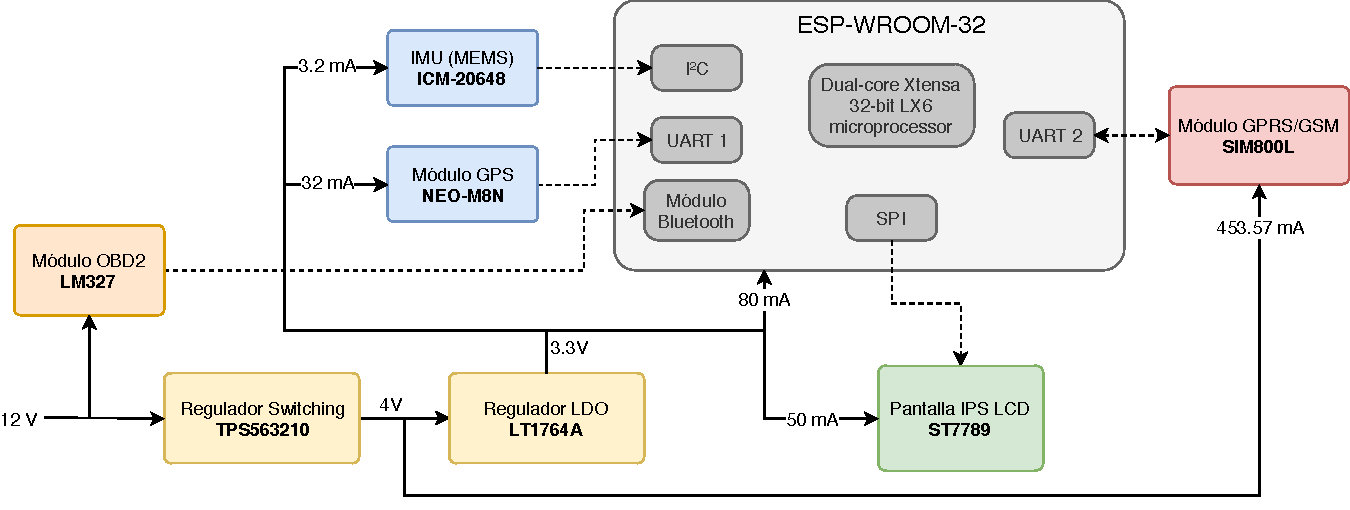
\includegraphics[width=\textwidth]{Bloques_total.pdf}}%
\caption{Diagrama de bloques del sistema con corrientes promedio.}
\label{fig:Bloques_comp}
\end{figure}



\subsection{Diagramas electrónicos}
En esta sección se presentarán las conexiones de los componente seleccionados anteriormente. Estas conexiones se realizaron siguiendo las recomendaciones que se encuentran en las hojas de datos de cada componente.

\subsubsection{IMU}
Se realiza el esquemático (Fig.~\ref{fig:IMU_esquem}) mostrando las conexiones necesarias para poder alimentar al módulo y para que este pueda comunicarse con el microcontrolador. Se establece el voltaje de alimentación y el voltaje lógico a \SI{3.3}{V}. En la hoja de datos \cite{ICM20648} se recomiendan los valores de los capacitores y se conectan los pines necesarios para poder implementar el protocolo de comunicación I\textsuperscript{2}C. El pin 9 se conecta a GND para establecer la dirección I\textsuperscript{2}C a b1101000.

\begin{figure}[htb!]
\centering
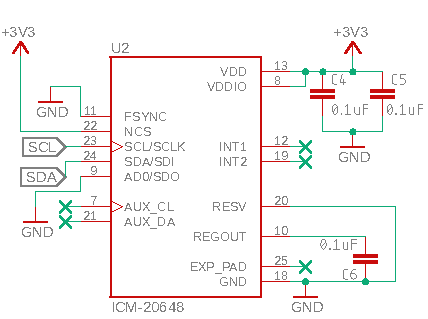
\includegraphics[width=\textwidth]{IMU_esquem.pdf}
\caption{Esquemático del módulo ICM-20648.}
\label{fig:IMU_esquem}
\end{figure}




\subsubsection{Módulo GPS}
Se realiza el esquemático (Fig.~\ref{fig:GPS_esquem}) de las conexiones necesarias para alimentar al módulo e implementar la comunicación con el microcontrolador. En este caso se alimenta al módulo con \SI{3.3}{V} y se implementa comunicación serial con el microcontrolador. Además se tiene un conector SMA para poder conectar una antena externa y también se cuenta con una batería de \SI{3}{V}, con una capacidad de \SI{5}{mAh} según \cite{MS621FE}.

Esta batería, que se recomienda en la hoja de datos \cite{GPS}, se encargará de mantener activo al módulo GPS en modo de bajo consumo durante la noche cuando la fuente de voltaje principal este desconectada. Esto se quiere hacer debido a que el GPS encontrará la posición de una forma más rápida si se mantiene activo. En cambio, cuando se apaga y se vuelve a encender se le llama "encendido en frío" y toma más tiempo.

\begin{figure}[htbp!]
\centering
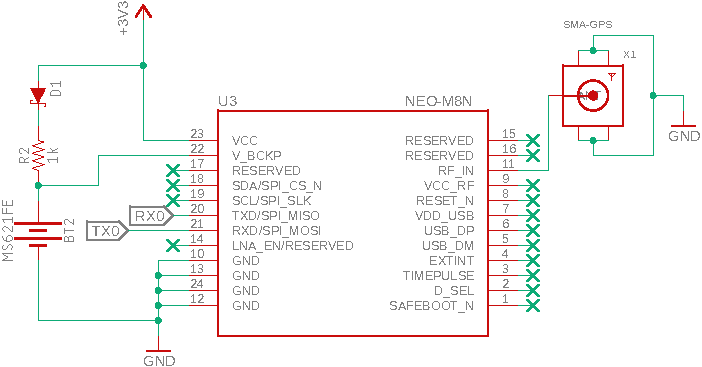
\includegraphics[width=\textwidth]{GPS_esquem.pdf}
\caption{Esquemático del módulo NEO-M8N.}
\label{fig:GPS_esquem}
\end{figure}



\subsubsection{Módulo GPRS/GSM}
A partir de los parámetros mencionados en la Tabla~\ref{diag:SIM} y de la hoja de datos \cite{SIM800L} se realiza el esquemático (Fig.~\ref{fig:GSM_esquem}) de las conexiones necesarias para alimentar al módulo e implementar la comunicación con el microcontrolador.

\begin{figure}[htb!]
\centering
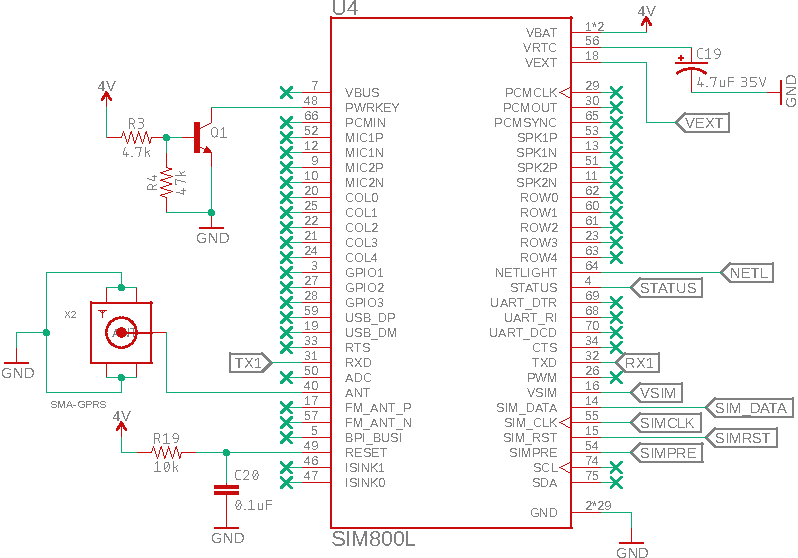
\includegraphics[width=\textwidth]{GSM_esquem.pdf}
\caption{Esquemático del módulo SIM800L.}
\label{fig:GSM_esquem}
\end{figure}

En este caso el módulo es alimentado con \SI{4}{V} y se usará comunicación serial. Los capacitores elegidos son recomendaciones de la hoja de datos \cite{SIM800L} al igual que el transistor que cumplirá la función de encender y apagar correctamente el módulo.

Además se necesita de un módulo que lea una tarjeta SIM. En la Fig.~\ref{fig:GSM_SIM_esquem} se muestra el esquemático de este módulo, el lector de tarjetas SIM (SIM8055).

\begin{figure}[htbp!]
\centering
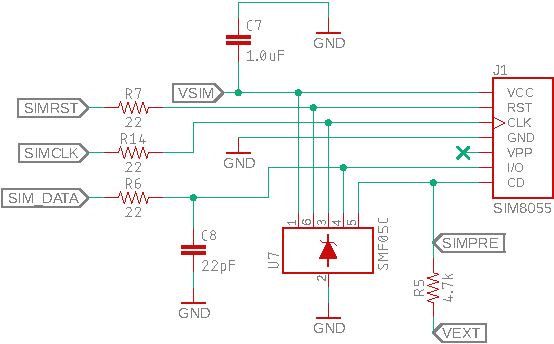
\includegraphics[width=\textwidth]{GSM_SIM_esquem.pdf}
\caption{Esquemático del módulo SIM8055.}
\label{fig:GSM_SIM_esquem}
\end{figure}

Por último, se tiene en la Fig.~\ref{fig:GSM_LED_esquem} el esquemático de la conexión de dos LEDs que servirán para indicar el estado de la conexión a Internet del módulo y también si este se encuentra encendido o no. Se usará un conector para cablear los LEDs ya que estos no se encontrarán soldados a la PCB porque se necesitan en una posición específica del case del dispositivo.

\begin{figure}[htbp!]
\centering
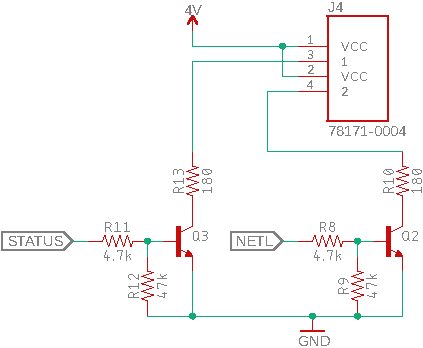
\includegraphics[width=0.7\textwidth]{GSM_LED_esquem.pdf}
\caption{Esquemático las los indicadores LED.}
\label{fig:GSM_LED_esquem}
\end{figure}



\subsubsection{Pantalla}
La pantalla se colocará fuera del case donde estará el PCB por lo que se usarán borneras para conectar los pines necesarios al microcontrolador, como indica la Fig.~\ref{fig:DISPLAY_esquem}. Se usa el protocolo SPI para comunicarse con el microcontrolador y se alimenta a la pantalla con \SI{3.3}{V}. Además se usan solo 8 pines ya que estos son los únicos necesarios para controlar la pantalla.

\begin{figure}[htbp!]
\centering
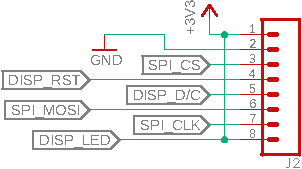
\includegraphics[width=0.6\textwidth]{DISPLAY_esquem.pdf}
\caption{Esquemático bornera para conectar la pantalla.}
\label{fig:DISPLAY_esquem}
\end{figure}


\subsubsection{Microcontrolador}
En la Fig.~\ref{fig:ESP_esquem} se muestra el esquemático del microcontrolador y su alimentación. En la hoja de datos \cite{Esp32_Hardware} se recomienda usar los capacitores que se encuentran conectados al microcontrolador y se muestran también todas las conexiones de los módulos anteriores; 1 conexión I\textsuperscript{2}C, 2 conexiones seriales y 1 conexión SPI.

\begin{figure}[hbtp!]
\centering
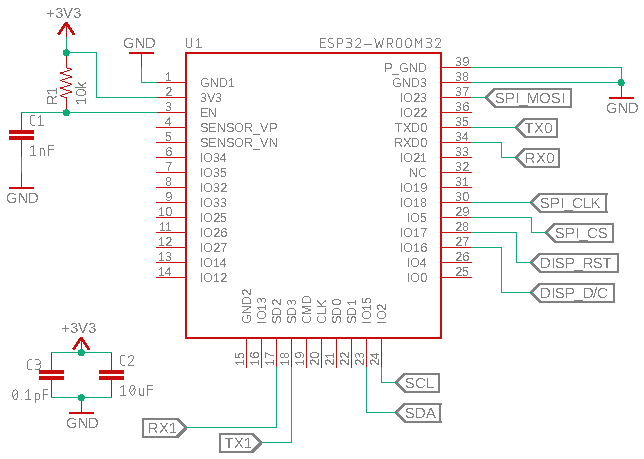
\includegraphics[width=\textwidth]{ESP32_esquem.pdf}
\caption{Esquemático de la implementación del ESP-WROOM-32.}
\label{fig:ESP_esquem}
\end{figure}


\subsubsection{Regulador swtiching}
En la Fig.~\ref{fig:esquem_switching} se puede observar la selección de los componentes externos al TPS563210 usados para obtener una salida de \SI{4}{V} de una fuente de \SI{12}{V}. El primer paso para seleccionar estos componentes fue determinar el voltaje de salida requerido (\SI{4}{V}). En \cite{TPS563210} se tiene que el V\textsubscript{out} seguirá la Ecuación~\ref{eq:vout}.
\begin{figure}[hbtp!]
\centering
\makebox[\textwidth][c]{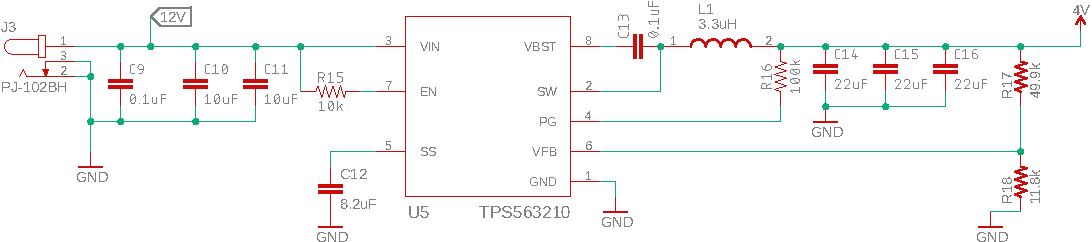
\includegraphics[width=\textwidth]{Switching.pdf}}%
\caption{Esquemático de la implementación del TPS563210.}
\label{fig:esquem_switching}
\end{figure}

\begin{equation}
    V_{out}=0.765\times(1+\frac{R_{17}}{R_{18}})
    \label{eq:vout}
\end{equation}

Para asegurar que $V_{out}=\SI{4}{V}$ se usan resistencias de la serie E96 (con 1\% de tolerancia en su valor). Los valores de $R_{17}$ y $R_{18}$ que cumplen con esta ecuación son $R_{17}=\SI{49.9}{k\ohm}$ y $R_{17}=\SI{11.8}{k\ohm}$.

Luego se recomienda en \cite{TPS563210} usar una inductancia de valor $L_1=\SI{3.3}{\micro H}$ y el IC usa una frecuencia de $f_{SW}=\SI{650}{kHz}$. Además se necesita el valor máximo que el voltaje de entrada V\textsubscript{in} puede tomar, que en este caso será $V_{in}=\SI{16}{V}$ (Esto es debido a fluctuaciones en el voltaje de la batería). Con estos valores se puede determinar los parámetros $Il_{P-P}$, $Il_{PEAK}$,  $I_{LO(RMS)}$ y $I_{CO}$ con las ecuaciones:
\begin{align}
Il_{P-P}&=\frac{V_{out}}{V_{in(MAX)}}\times\frac{V_{in(MAX)}-V_{OUT}}{L_O\times f_{SW}} \label{eq:current1}\\
Il_{PEAK}&=I_{o}+\frac{Il_{P-P}}{2} \label{eq:current2}\\
I_{LO(RMS)}&=\sqrt{I_o^2+\frac{1}{12}Il_{P-P}^2} \label{eq:current3} \\
I_{CO}&=\frac{V_{out}\times (V_{in}-V_{out})}{\sqrt{12}\times V_{in}\times L_{O} \times f_{Sw}} \label{eq:current4}
\end{align}

El resultado de las Ecuaciones \ref{eq:current1}, \ref{eq:current2}, \ref{eq:current3} y \ref{eq:current4} son:
\begin{align*}
Il_{P-P}&=\SI{1.398}{A} &
Il_{PEAK}&=\SI{3.319}{A}&
I_{LO(RMS)}&=\SI{2.79}{A} &
I_{CO(RMS)}&=\SI{0.02}{A}
\end{align*}

Se selecciona entonces el inductor CLF7045NIT-3R3N-D de \SI{3.3}{\micro H} que soporta los parámetros mencionados anteriormente \cite{Inductor} y 3 capacitores C3216X5R0J226M en la salida de \SI{22}{\micro F}  que soporta hasta \SI{4}{A} RMS. Los capacitores de entrada y las demás resistencias se colocan por recomendación de \cite{TPS563210}.


\subsubsection{Regulador LDO}

En la Fig.~\ref{fig:LDO} se puede observar la selección de componentes externos y el esquemático propuesto para el LT1764A. Los capacitores C\textsubscript{17} y C\textsubscript{18} toman valores recomendados en la hoja de datos \cite{LT1764A}

\begin{figure}[hbtp!]
\centering
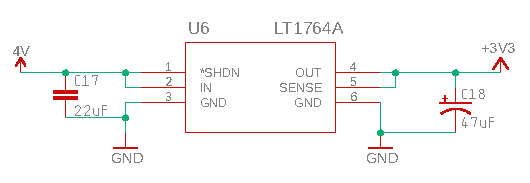
\includegraphics[width=\textwidth]{LDO.pdf}
\caption{Esquemático de la implementación del LT1764A.}
\label{fig:LDO}
\end{figure}









\subsection{Diseño del PCB}
A continuación se incluirá el diseño del PCB en el que irán todos los componentes antes mencionados. Como se aprecia en la Fig.~\ref{fig:Board}, el PCB cuenta con dos capas. La capa inferior cuenta con un plano de GND que ayudará no solo a conectar los componentes más fácilmente sino que es recomendado por algunos de los componentes como el SIM 800L \cite{SIM800L}.

\begin{figure}[hbtp!]
\centering
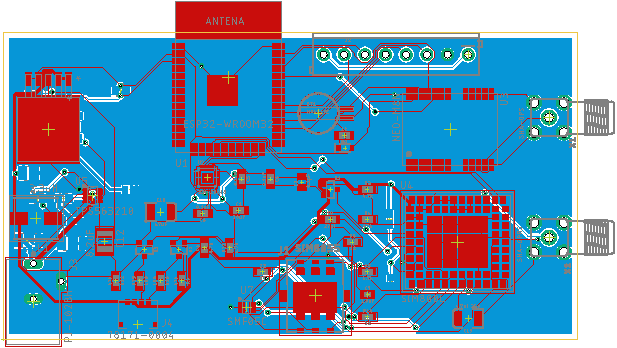
\includegraphics[width=\textwidth]{Board.pdf}
\caption{Diseño del PCB.}
\label{fig:Board}
\end{figure}


En la Fig.~\ref{fig:board_top} se puede apreciar la parte superior del PCB con sus dimensiones en mm y en la Fig.~\ref{fig:board_bottom} se aprecia la parte inferior

\begin{figure}[hbtp!]
\centering
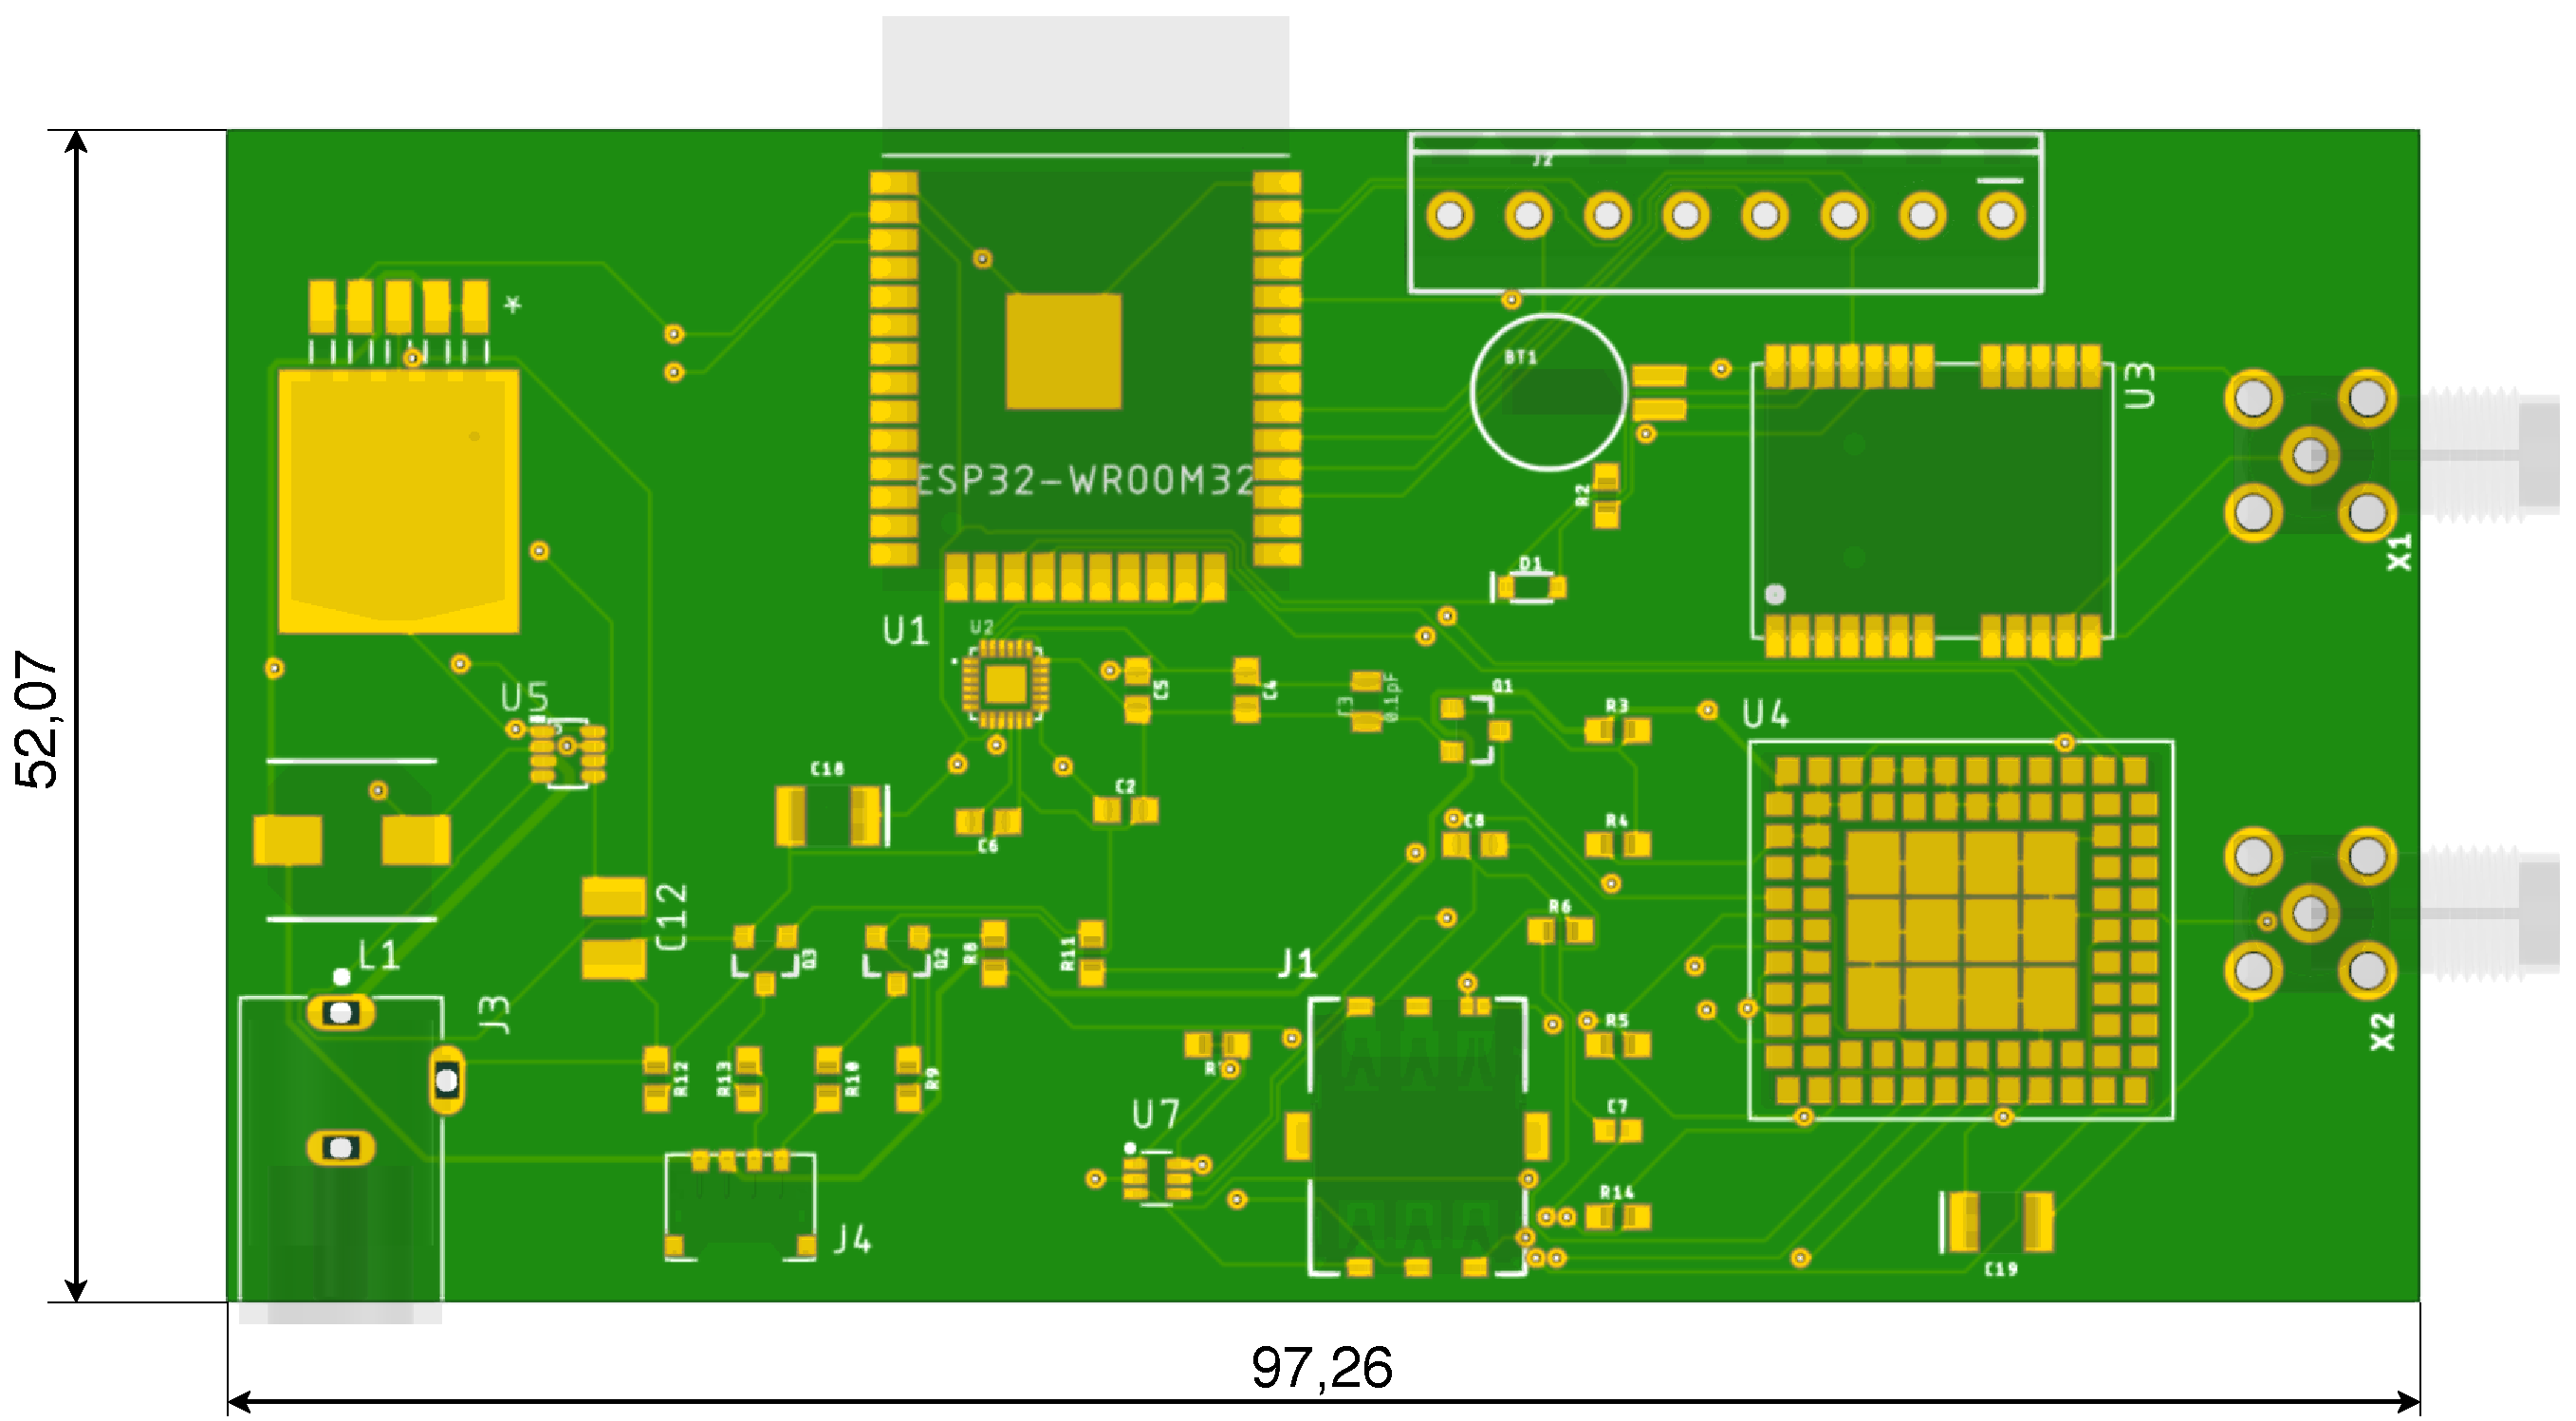
\includegraphics[width=\textwidth]{board_top_dim.pdf}
\caption{Parte superior del PCB.}
\label{fig:board_top}
\end{figure}

\begin{figure}[hbtp!]
\centering
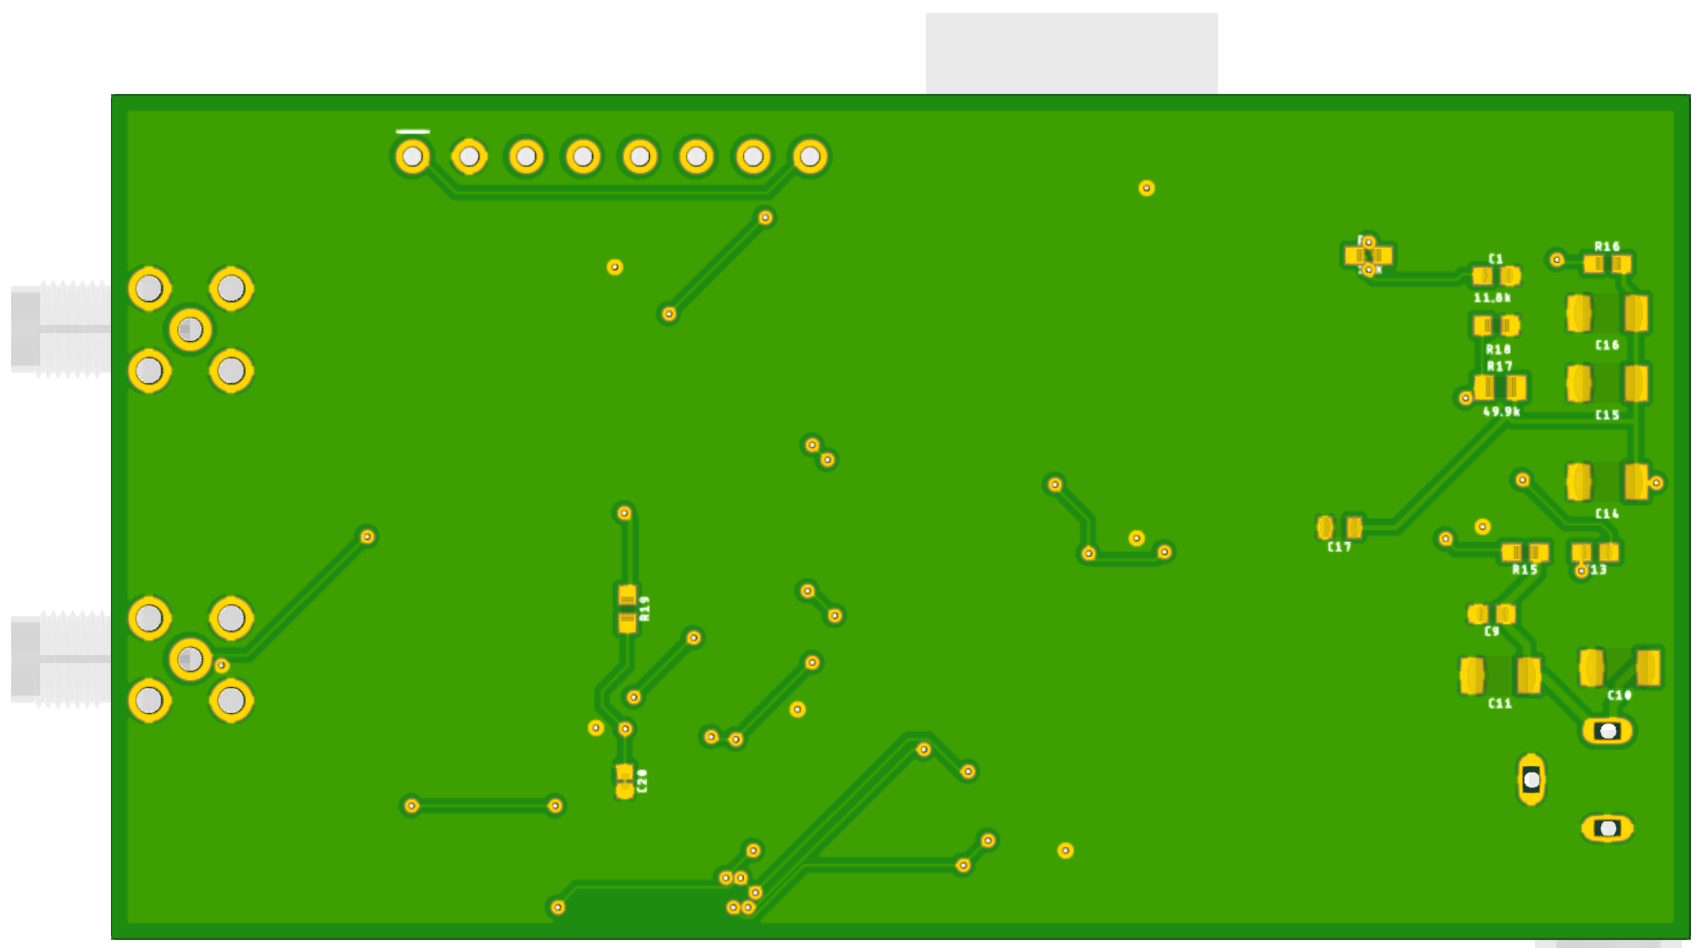
\includegraphics[width=\textwidth]{board_bottom.png}
\caption{Parte inferior del PCB.}
\label{fig:board_bottom}
\end{figure}

Se tuvo una consideración importante al escoger el ancho de las pistas que se encuentran en este PCB. Siguiendo la Fig.~\ref{fig:bloques_alim}, en donde se pueden ver las corrientes máximas que se alcanzarán. Se tienen pistas por donde pasarán \SI{2.6}{A}, \SI{2}{A} y \SI{0.62}{A}. Para poder elegir el ancho adecuadamente se utiliza la Ecuación~\ref{eq:width1} en dónde $I$ es la máxima corriente permisible, $\Delta T$ es el incremento de temperatura permisible y $A$ es la sección transversal de la pista.

\begin{equation}
    I = k\Delta T^{0.44}A^{0.725}
    \label{eq:width1}
\end{equation}

Si expresamos $A=Espesor\times Ancho$ Y despejamos $Ancho$, obtendríamos la Ecuación~\ref{eq:width2}

\begin{equation}
    Ancho = \left(\frac{I}{k\Delta T^{0.44}}\right)^{\frac{1}{0.725}}\times \frac{1}{Espesor}
    \label{eq:width2}
\end{equation}


Al usar la Ecuación~\ref{eq:width2} con $\Delta T=\SI{20}{\celsius}$, y un espesor de pista de \SI{1}{oz/ft^2} se tienen los mínimos anchos de pista necesarios para cada corriente mencionada. Los resultados se observan en la Tabla~\ref{diag:traces_width}. Sin embargo, estos son solo los anchos mínimos. Es por eso que para una corriente de \SI{620}{mA} o menor se usará un ancho de pista de \SI{10}{mil} por defecto y de \SI{6}{mil} para soldar los pads del SIM 800L.

\bgroup
\def\arraystretch{1.5}%  1 is the default, change whatever you need
\begin{table}[htbp!]
\centering
\caption[Anchos de pista mínimos]{Anchos de pista mínimos.}
\begin{tabular}{@{}ll@{}}
\toprule
Corriente máxima & Ancho mínimo \\ \midrule
\SI{2.6}{A} & \SI{29}{mil} \\
\SI{2}{A} & \SI{20.2}{mil} \\
\SI{620}{mA} & \SI{4}{mil} \\ \bottomrule
\end{tabular}
\label{diag:traces_width}
\end{table}
\egroup

El PCB diseñado tiene componentes que exceden las dimensiones de la placa. Las dimensiones con componentes se puede apreciar en las Figuras \ref{fig:board_top_con},  \ref{fig:board_bottom_con} y \ref{fig:board_side_con}

\begin{figure}[hbtp!]
\centering
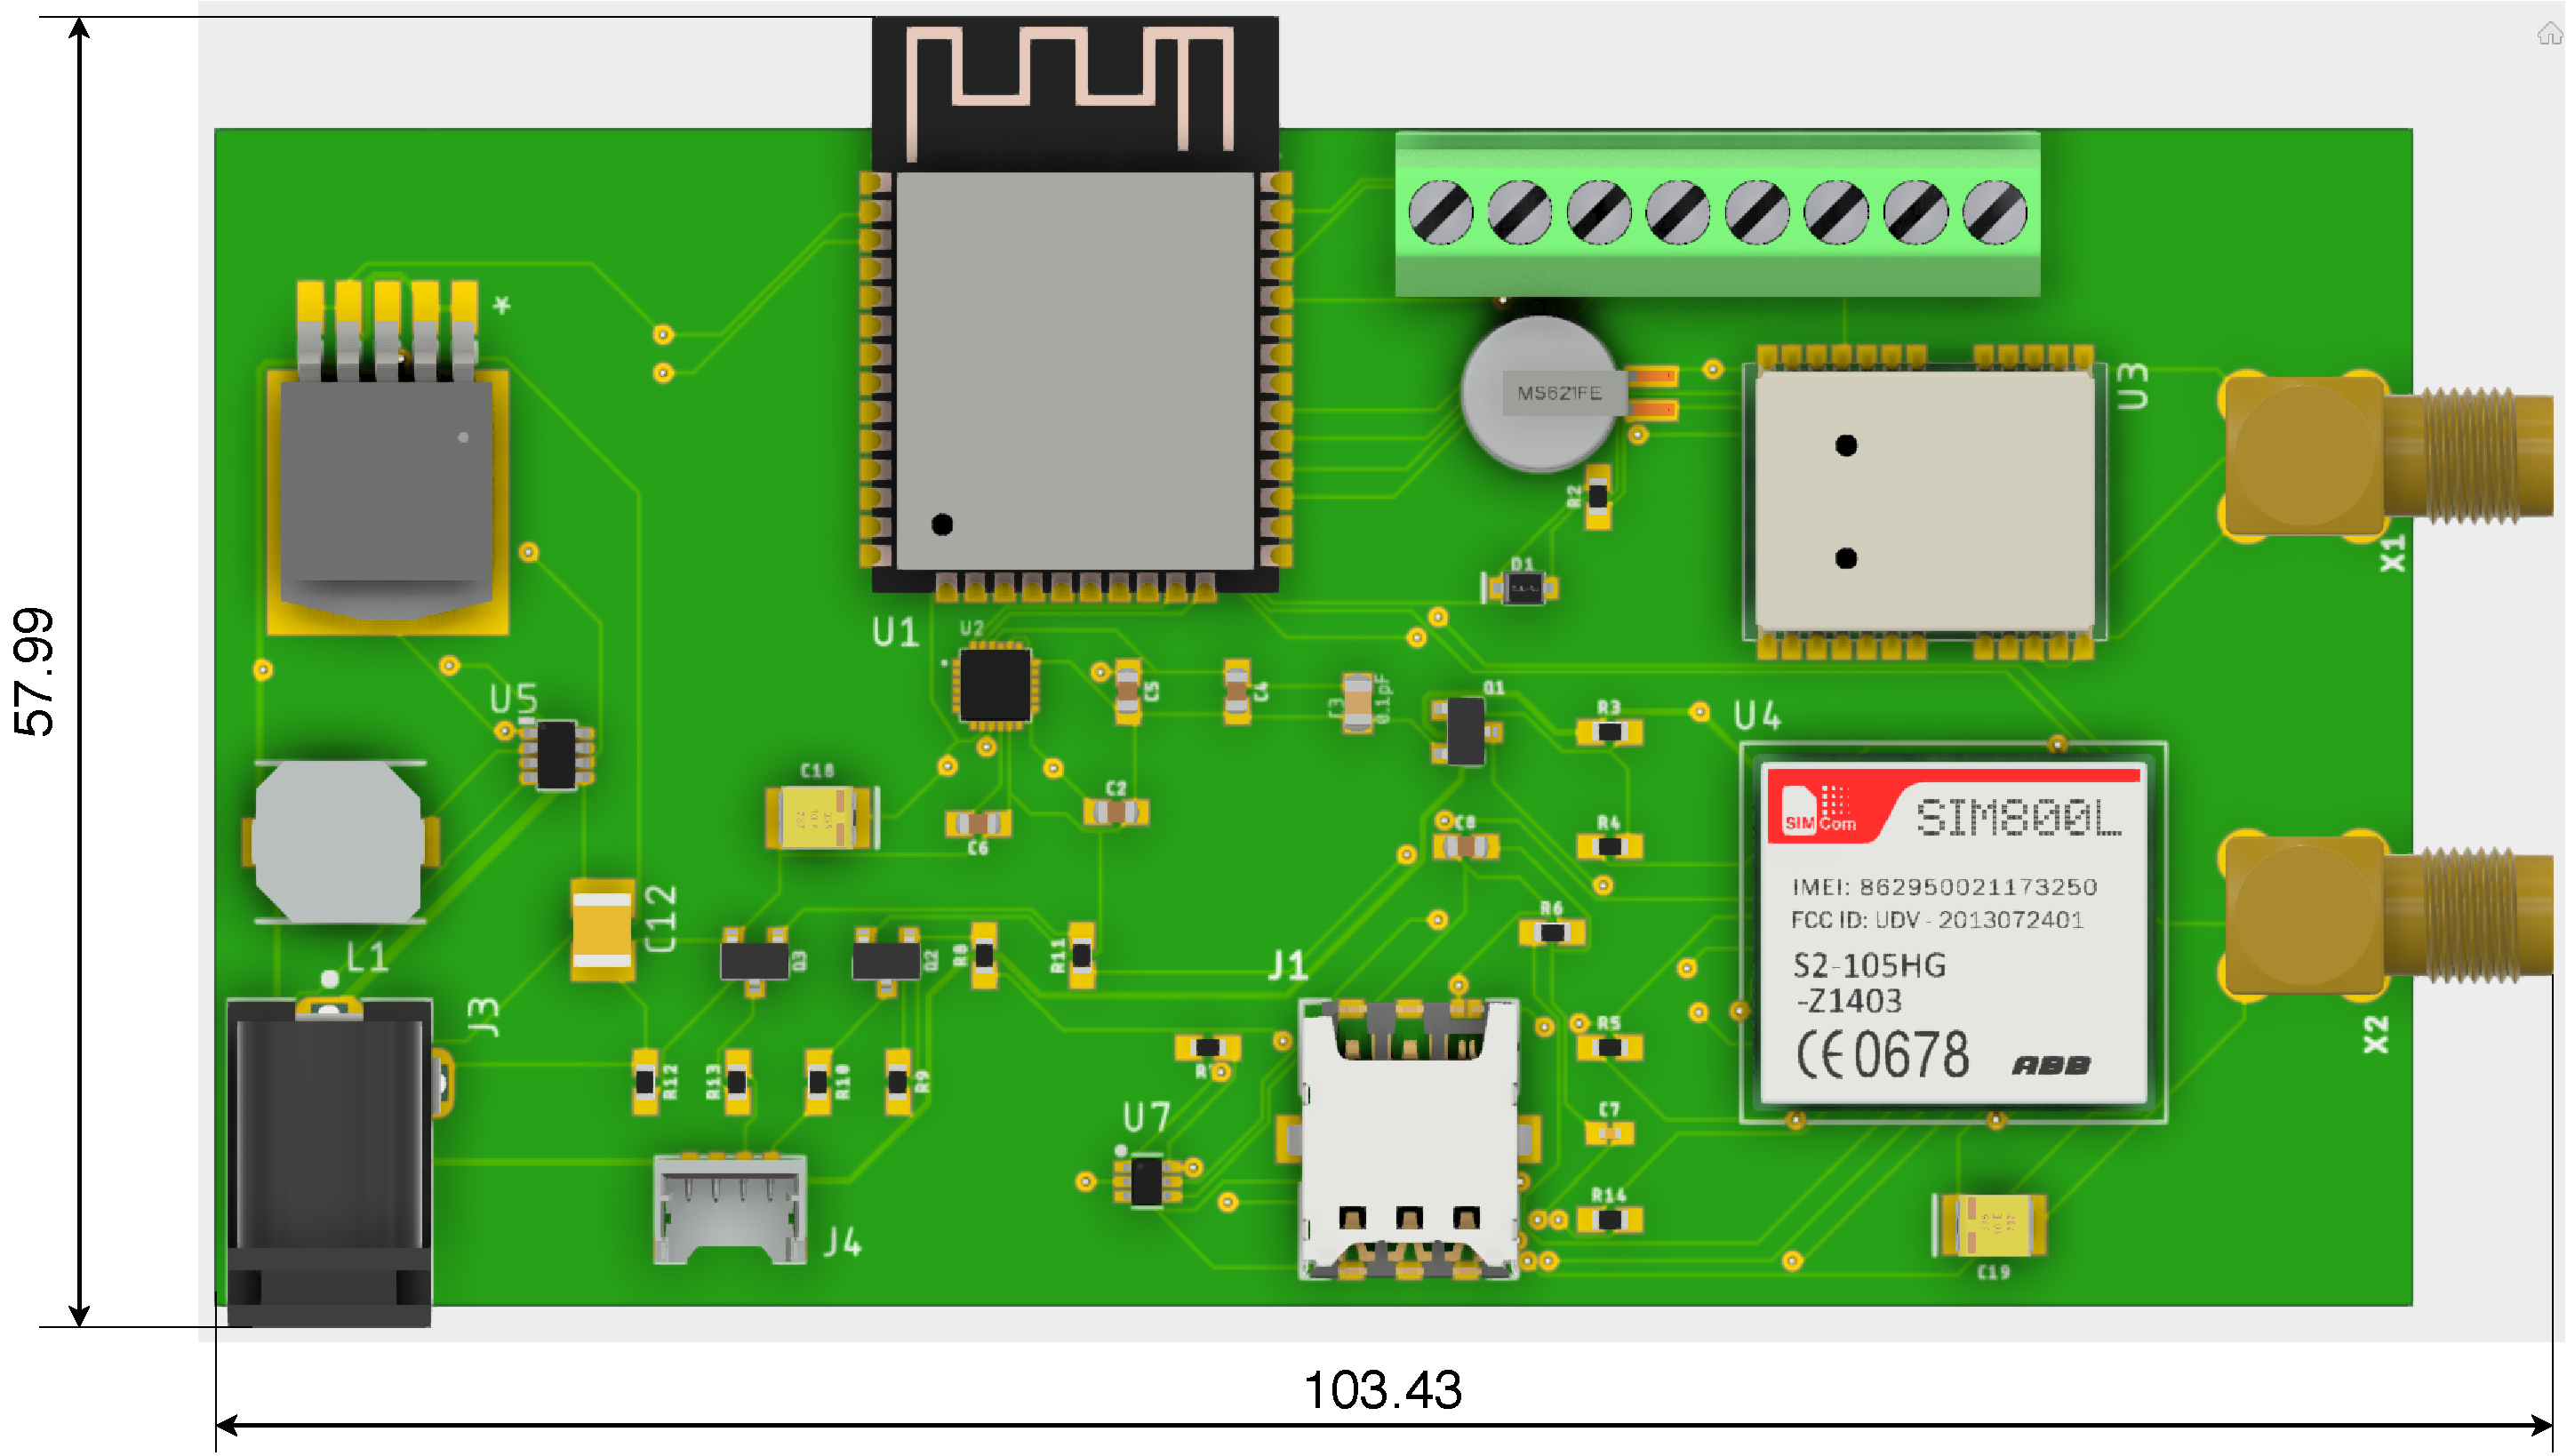
\includegraphics[width=\textwidth]{board_top_com_dim.pdf}
\caption{Parte superior del PCB con componentes.}
\label{fig:board_top_con}
\end{figure}

\begin{figure}[hbtp!]
\centering
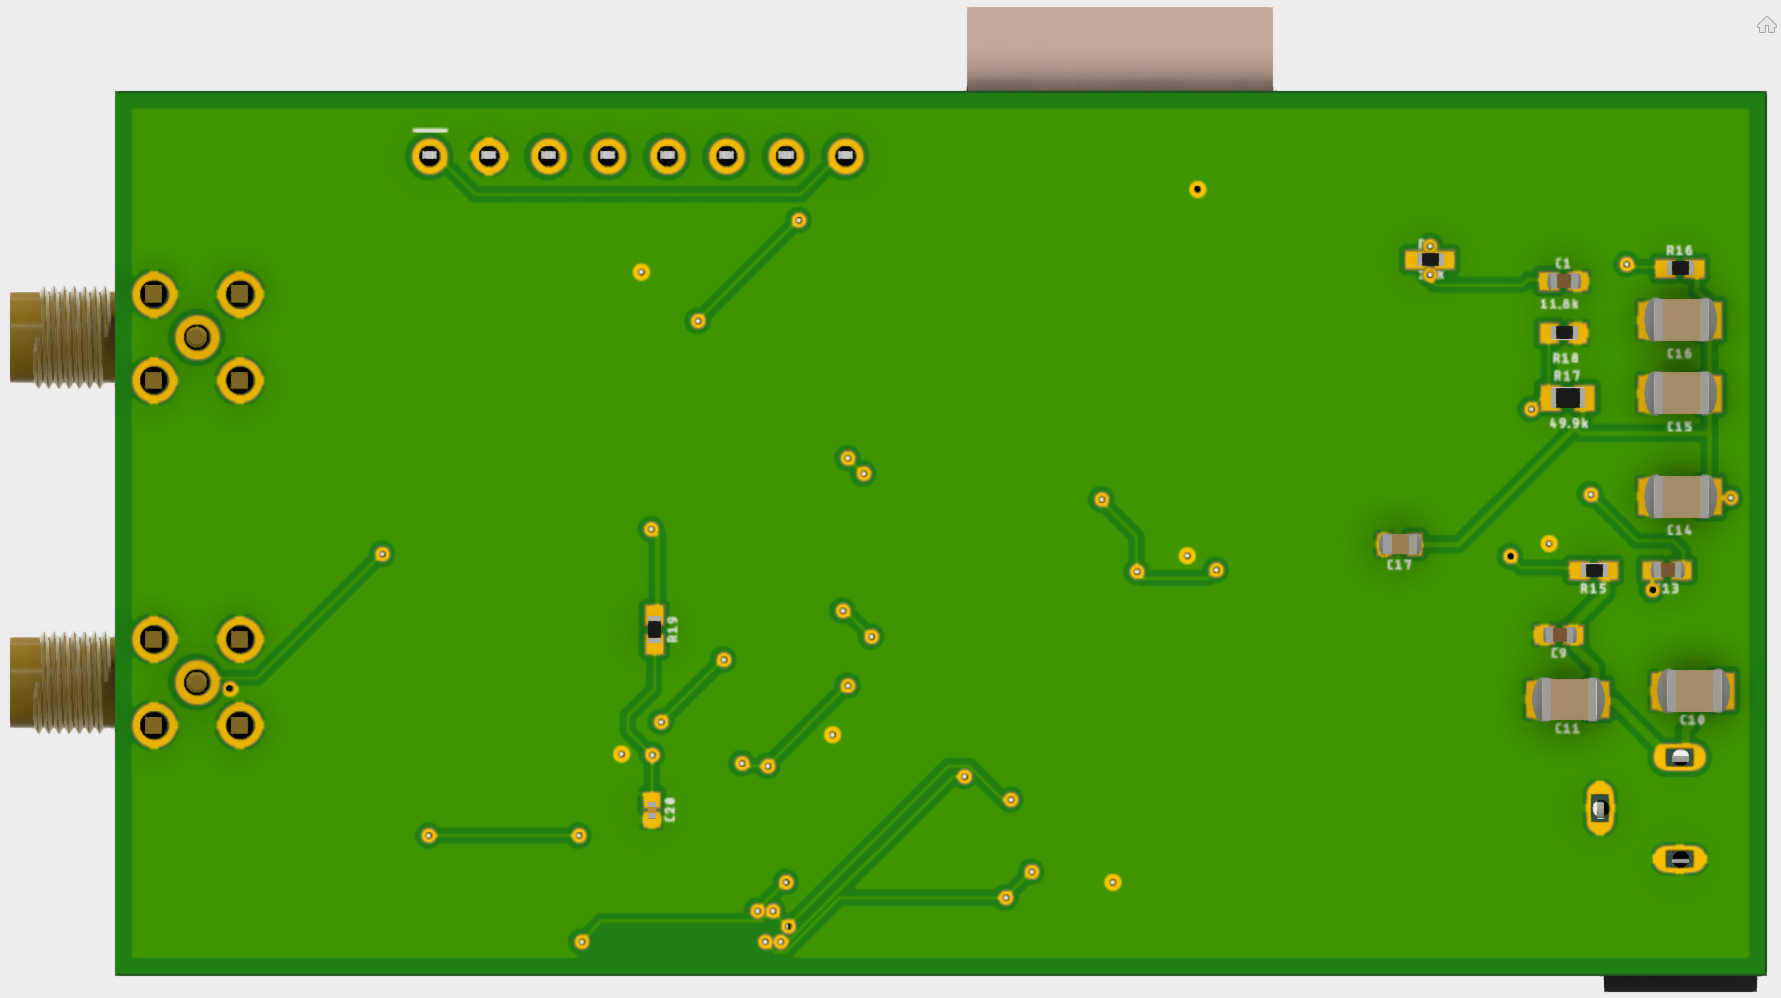
\includegraphics[width=\textwidth]{board_com_bottom.png}
\caption{Parte inferior del PCB con componentes.}
\label{fig:board_bottom_con}
\end{figure}

\begin{figure}[hbtp!]
\centering
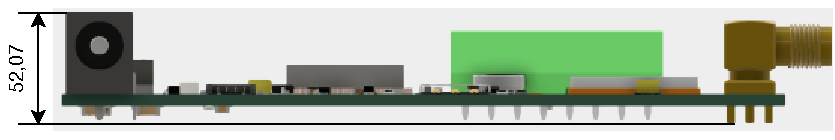
\includegraphics[width=\textwidth]{board_side_dim.pdf}
\caption{Vista lateral del PCB.}
\label{fig:board_side_con}
\end{figure}


\section{Diseño mecánico}

En este capítulo se describirá el proceso de diseño del case principal y de la pantalla, además de los ensambles entre ellos. La lista de planos se puede encontrar en el Anexo \ref{anexo:planos}.

\subsection{Diseño del Case Principal}

El PCB antes diseñado tiene las dimensiones $\SI{58}{mm} \times \SI{103.43}{mm} \times \SI{14.9}{mm}$. Se diseña entonces un case que pueda alojar esta placa electrónica y que permita acceder a las interfaces que posee (Conexión de alimentación, ranura de Nano SIM y conectores SMA). El case diseñado tendrá las dimensiones $\SI{63}{mm} \times \SI{108}{mm} \times \SI{28}{mm}$ y además de las interfaces mencionadas anteriormente tendrá también 2 indicadores LED que mostraran el encendido del dispositivo y su conexión a Internet. Todos estos elementos se pueden observar en las Fig.~\ref{fig:exploded}.



\begin{figure}[hbt!]
\centering
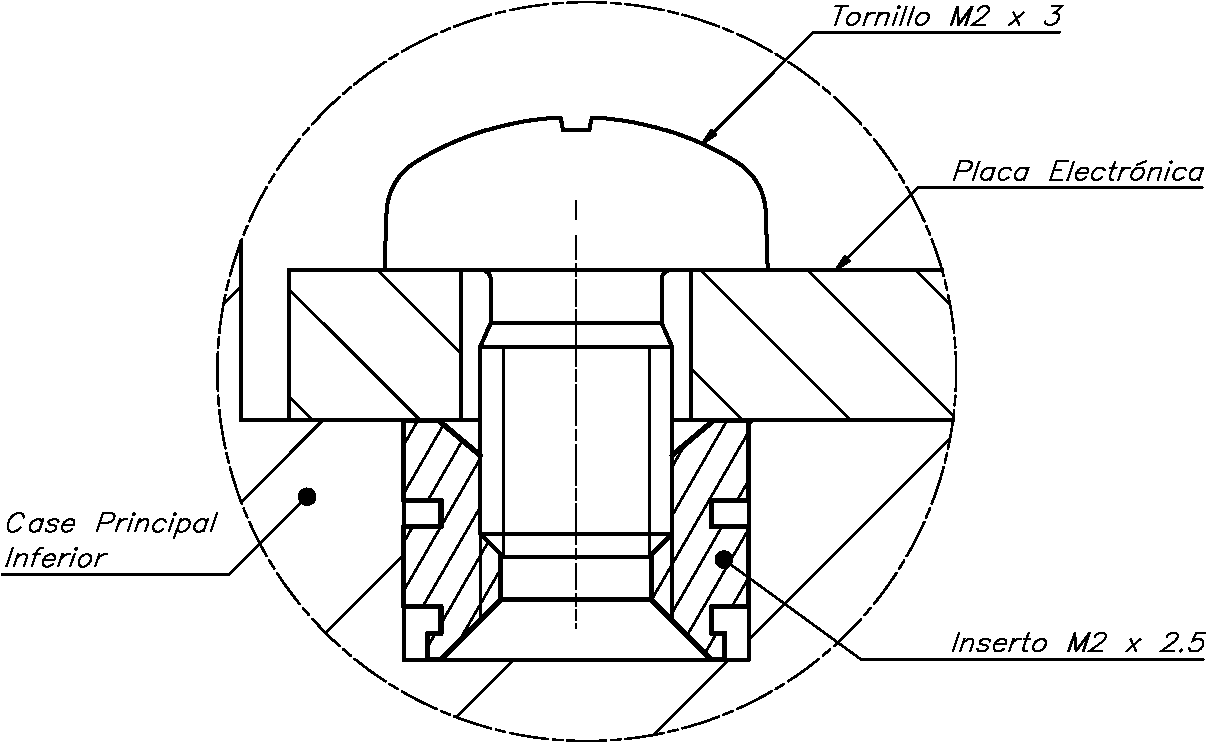
\includegraphics[width=0.8\textwidth]{union_atornillada.pdf}
\caption{Unión de la tarjeta electrónica con el case.}
\label{fig:ensamble_principal}
\end{figure}


\newpage

Este case cuenta con dos partes, una superior y otra inferior. En la inferior se ensamblará la tarjeta electrónica vista en el capítulo anterior. El ensamble (Fig.~\ref{fig:ensamble_principal}) se realizará usando una unión atornillada de un Tornillo M2 x 3 y un Inserto M2 x 2.5 que se coloca en un agujero en el case principal inferior.Este  inserto se puede observar en la Fig.~\ref{fig:insert} y esta diseñado para ser usado en plásticos.

\vspace{5mm}

\begin{figure} [hbt!]
\centering
\begin{minipage}{.5\textwidth}
  \centering
  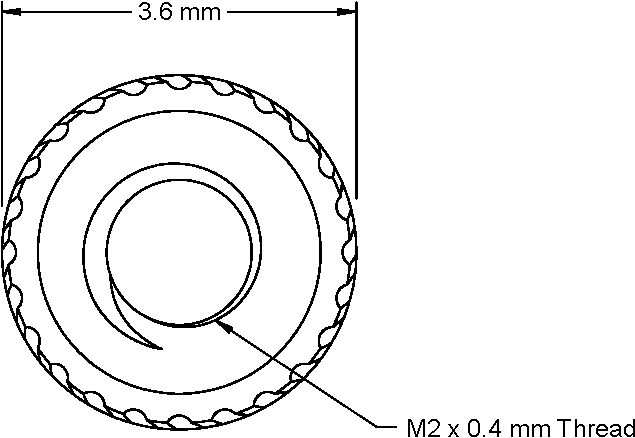
\includegraphics[width=.9\linewidth]{insert_1.pdf}
\end{minipage}%
\begin{minipage}{.5\textwidth}
  \centering
  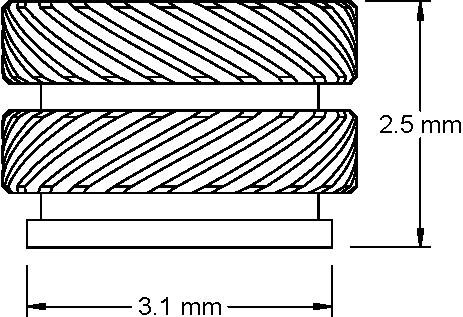
\includegraphics[width=.7\linewidth]{insert_2.pdf}
\end{minipage}
\caption{Inserto M2 x 2.5 para plástico.}
\label{fig:insert}
\end{figure}

Luego que la placa electrónica esta correctamente sujeta, se ensambla la parte superior del case. Para este ensamble se utilizan unas pestañas que encajarán entre si para facilitar el posicionamiento de las piezas y "snap fits" para la sujeción de las dos piezas. Esto se puede observar en la Fig.~\ref{fig:union-case_principal}.

Para el diseño de estás conexiones se tuvo en cuenta una separación de \SI{0.2}{mm} en las pestañas para asegurar que encajarán una con otra y que existirá un poco de fricción luego de ser impresas. Además se considero también una separación de \SI{0.3}{mm} en los snap fits para asegurar su posicionamiento.

\vspace{5mm}

\begin{figure}[hbt!]
\centering
\begin{subfigure}{.5\textwidth}
  \centering
  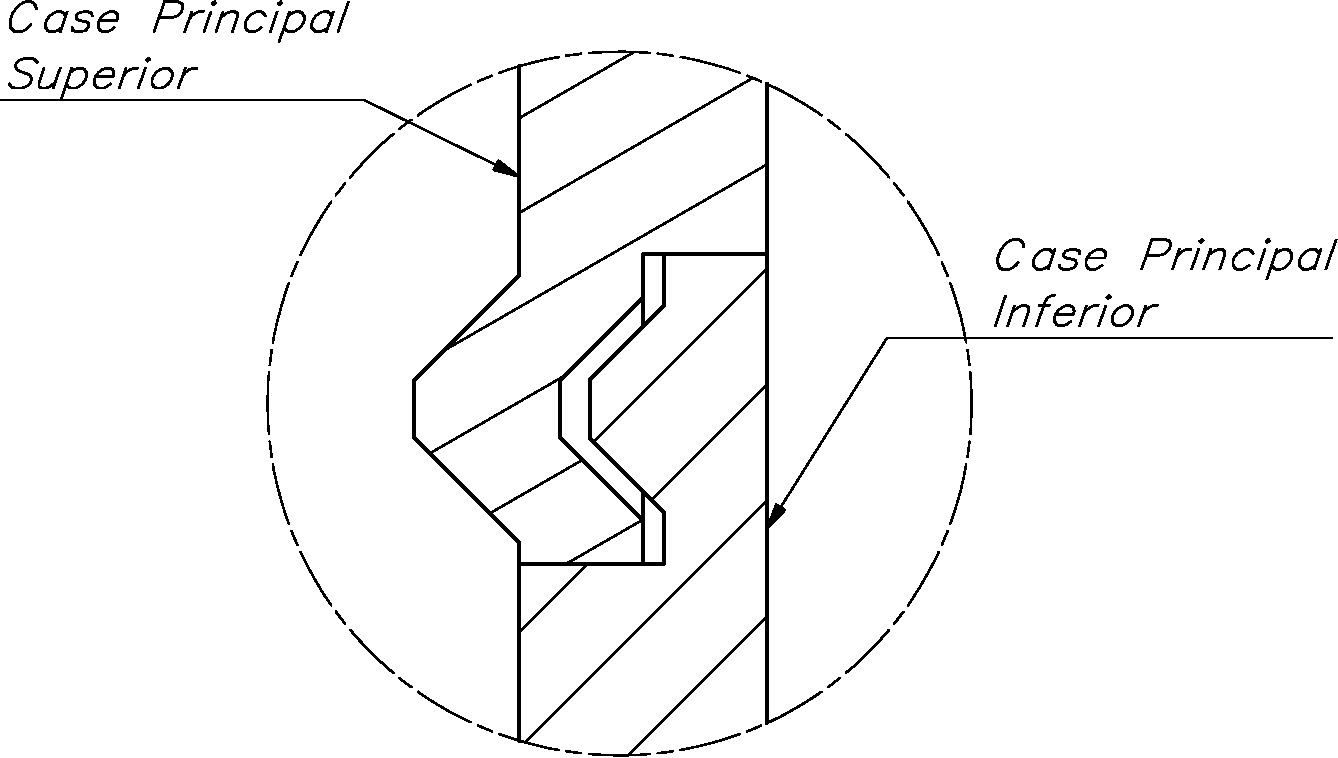
\includegraphics[width=\linewidth]{snap.pdf}
  \caption{Snap fits para la conexión}
  \label{fig:snaps_1}
\end{subfigure}%
\begin{subfigure}{.5\textwidth}
  \centering
  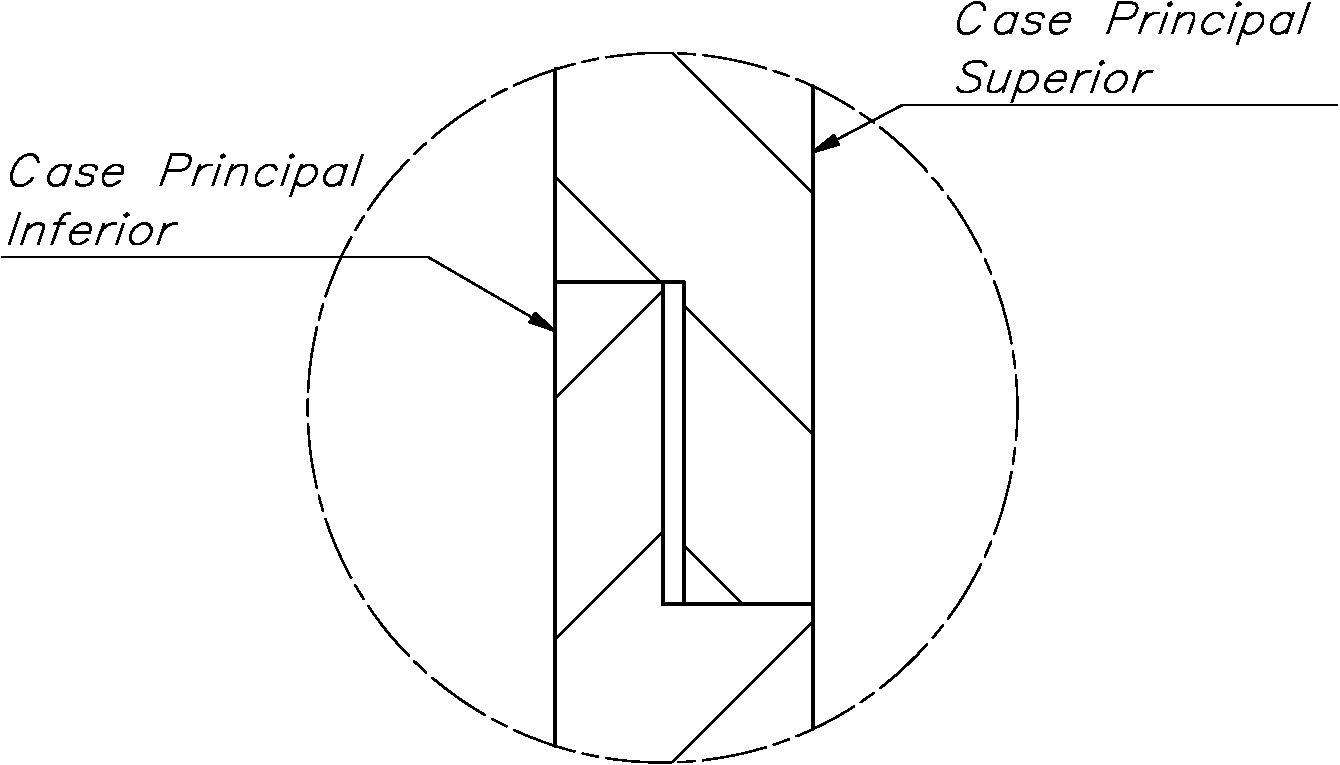
\includegraphics[width=0.9\linewidth]{lid.pdf}
  \caption{Pestañas para el posicionamiento}
  \label{fig:lid_1}
\end{subfigure}
\caption{Unión entre la parte superior e inferior del Case Principal}
\label{fig:union-case_principal}
\end{figure}

\newpage
\begin{figure}[hbt!]
\centering
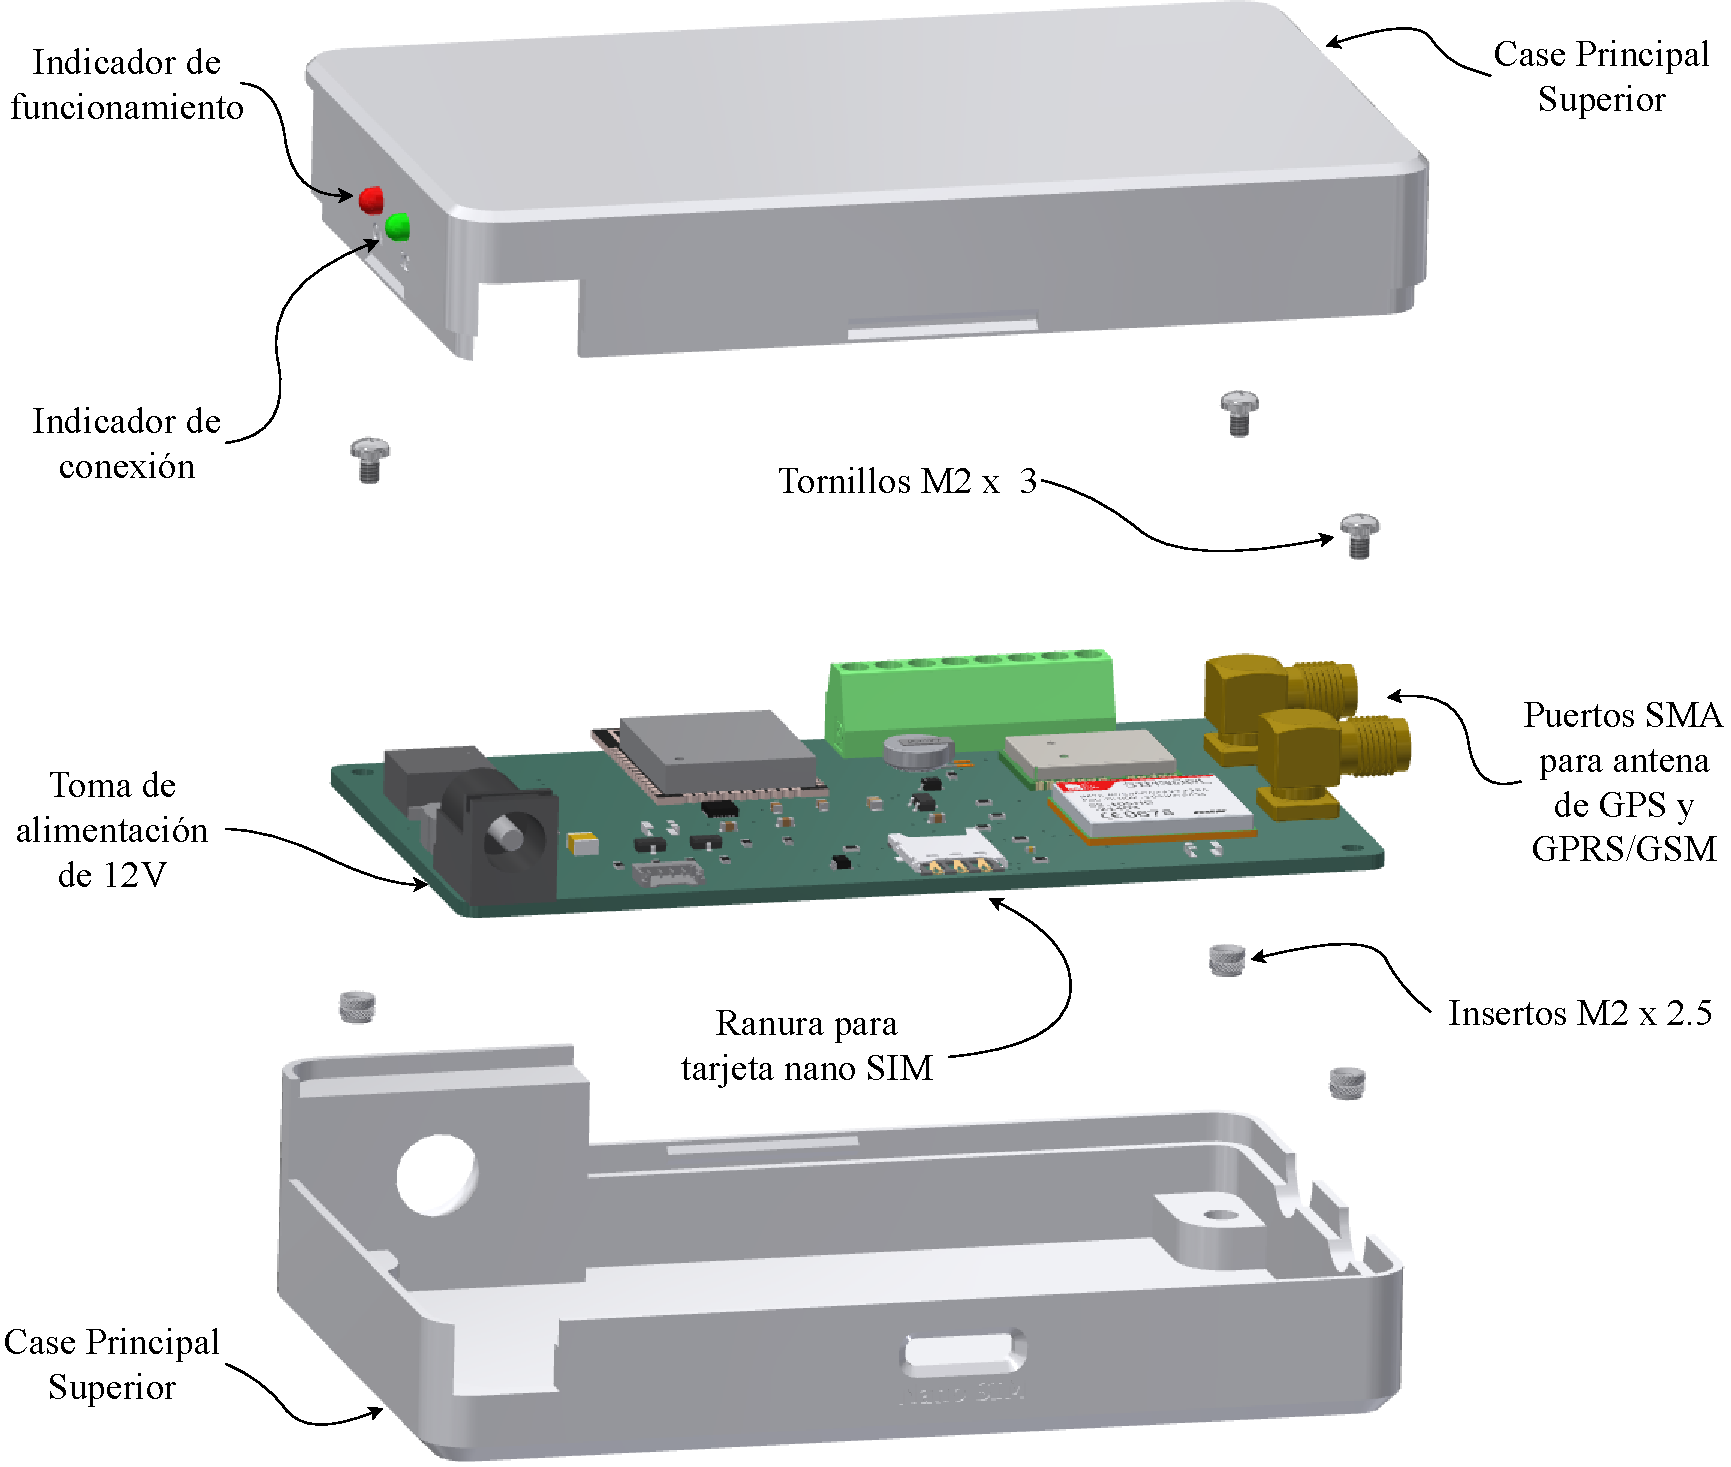
\includegraphics[width=\textwidth]{exploded.pdf}
\caption{Vista de explosión del case principal.}
\label{fig:exploded}
\end{figure}



%El case se diseñó teniendo en cuenta las limitaciones al usar ABS

%olerancias de impresión 3D de \SI{0.5}{mm} para que las piezas encajen sin problemas. El case se divide en dos partes. Estas partes encajan por forma y se atornillarán

%Para el ensamblaje de las dos partes del case se usan tornillos de rosca M2. Para la union atornillada se usan \textit{Inserts} metálicos para plástico que habilitan una rosca métrica.
%\subsection{Diseño del Case de la pantalla}
\subsection{Selección del brazo de la pantalla}

Para seleccionar el brazo que sujete la pantalla se tienen en cuenta dos requerimientos:
\vspace{-3mm}
\begin{itemize}
    \itemsep0pt
    \item La posición de la pantalla debe ser regulable por el conductor.
    \item Los cables tienen que poder ser conducidos a través del brazo hacia la pantalla
\end{itemize}

Se usarán entonces las mangueras a piezas de la marca \textit{Loc-Line} (Fig.~\ref{fig:brazo_1}). Estas mangueras se componen de múltiples piezas huecas, cada una se une a la siguiente por medio de una articulación de rótula. Entonces se crea uniones para poder conectar esta manguera con el case principal y con el case de la pantalla. En el caso del case principal se crea un agujero en donde entrará la rótula del primer elemento de la manguera (Fig.~\ref{fig:rotula_principal}) y en el caso de el case de la pantalla se creará un elemento que encajé en el agujero de rótula de la manguera (Fig.~\ref{fig:rotula_pantalla})


\begin{figure}[hbt!]
\centering
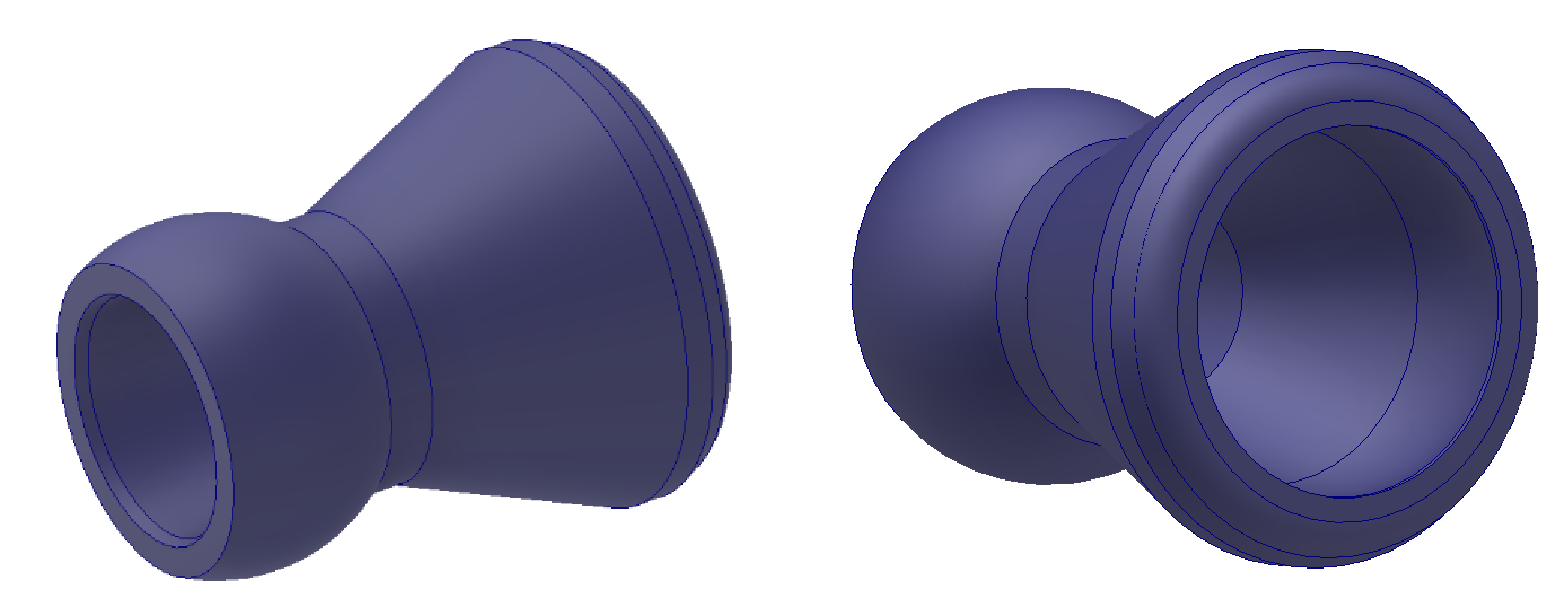
\includegraphics[width=0.8\textwidth]{brazo_1.pdf}
\caption{Elemento Loc-Line.}
\label{fig:brazo_1}
\end{figure}


\begin{figure}[hbt!]
\centering
\begin{subfigure}{.5\textwidth}
  \centering
  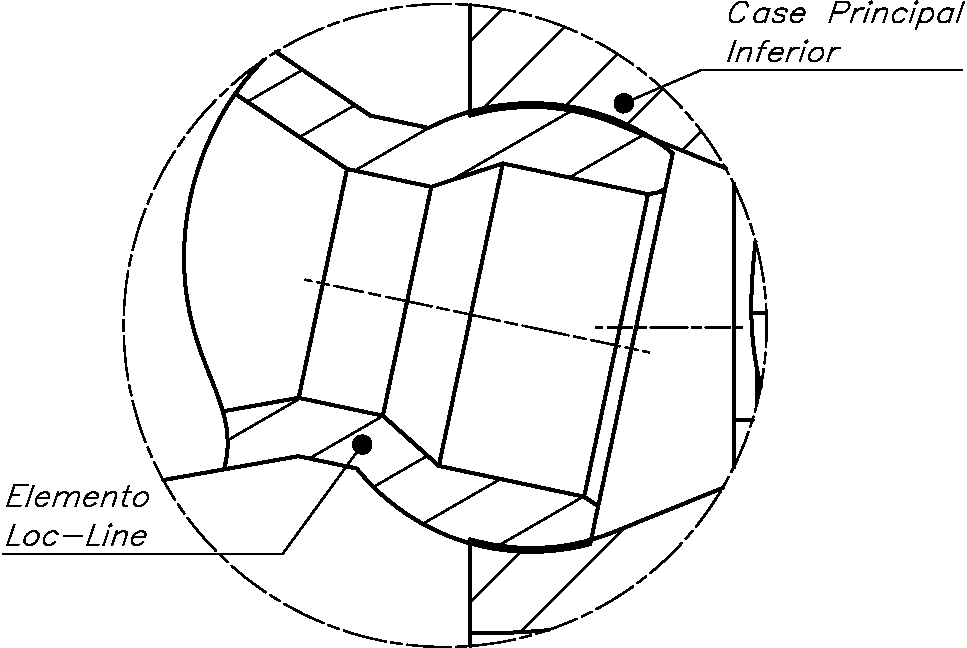
\includegraphics[width=0.9\linewidth]{rotula_principal.pdf}
  \caption{Rótula del case principal}
  \label{fig:rotula_principal}
\end{subfigure}%
\begin{subfigure}{.5\textwidth}
  \centering
  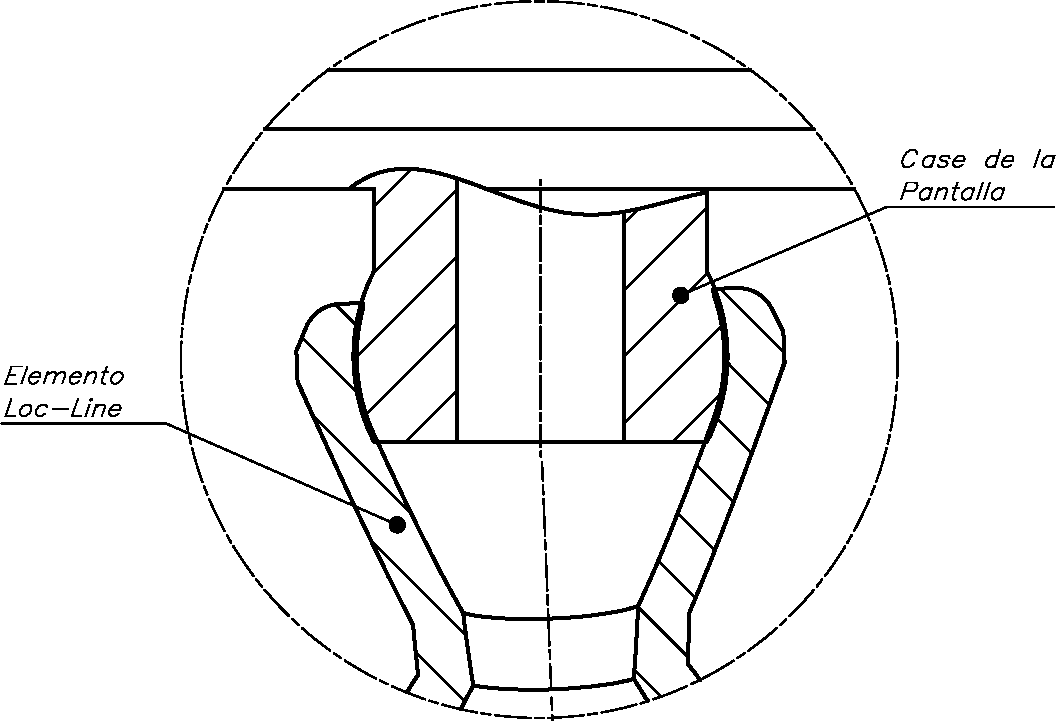
\includegraphics[width=\linewidth]{rotula_pantalla.pdf}
  \caption{Rótula del case de la pantalla}
  \label{fig:rotula_pantalla}
\end{subfigure}
\caption{Detalles del ensamble de los elementos Loc-Line con las cajas electrónicas}
\label{fig:rotulas}
\end{figure}


\subsection{Diseño del case de la pantalla}
El case de la pantalla se puede observar en la Fig.~\ref{fig:exploded_pantalla}. Este case de dimensiones $\SI{43}{mm} \times \SI{49}{mm} \times \SI{21}{mm}$ será impreso también en 3D. Para ensamblar las dos partes del case con la pantalla, se inserta la placa electrónica de la pantalla en un agujero con su misma forma en el case inferior de la pantalla. Luego la parte superior del case es ensamblada usando pestañas para el posicionamiento y snap fits para la sujeción.

\begin{figure}[hbt!]
\centering
\begin{subfigure}{.5\textwidth}
  \centering
  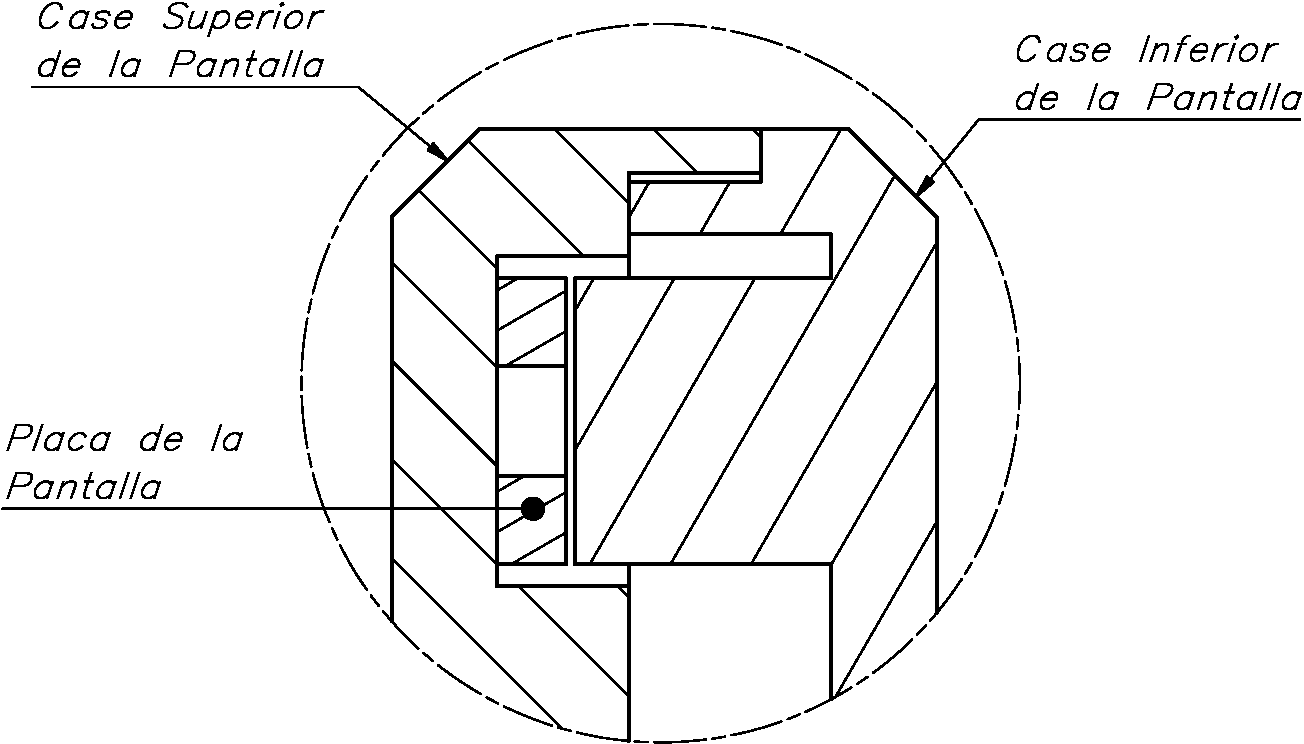
\includegraphics[width=0.9\linewidth]{union_pantalla.pdf}
  \caption{Unión del Case de la Pantalla}
  \label{fig:union_pantalla}
\end{subfigure}%
\begin{subfigure}{.5\textwidth}
  \centering
  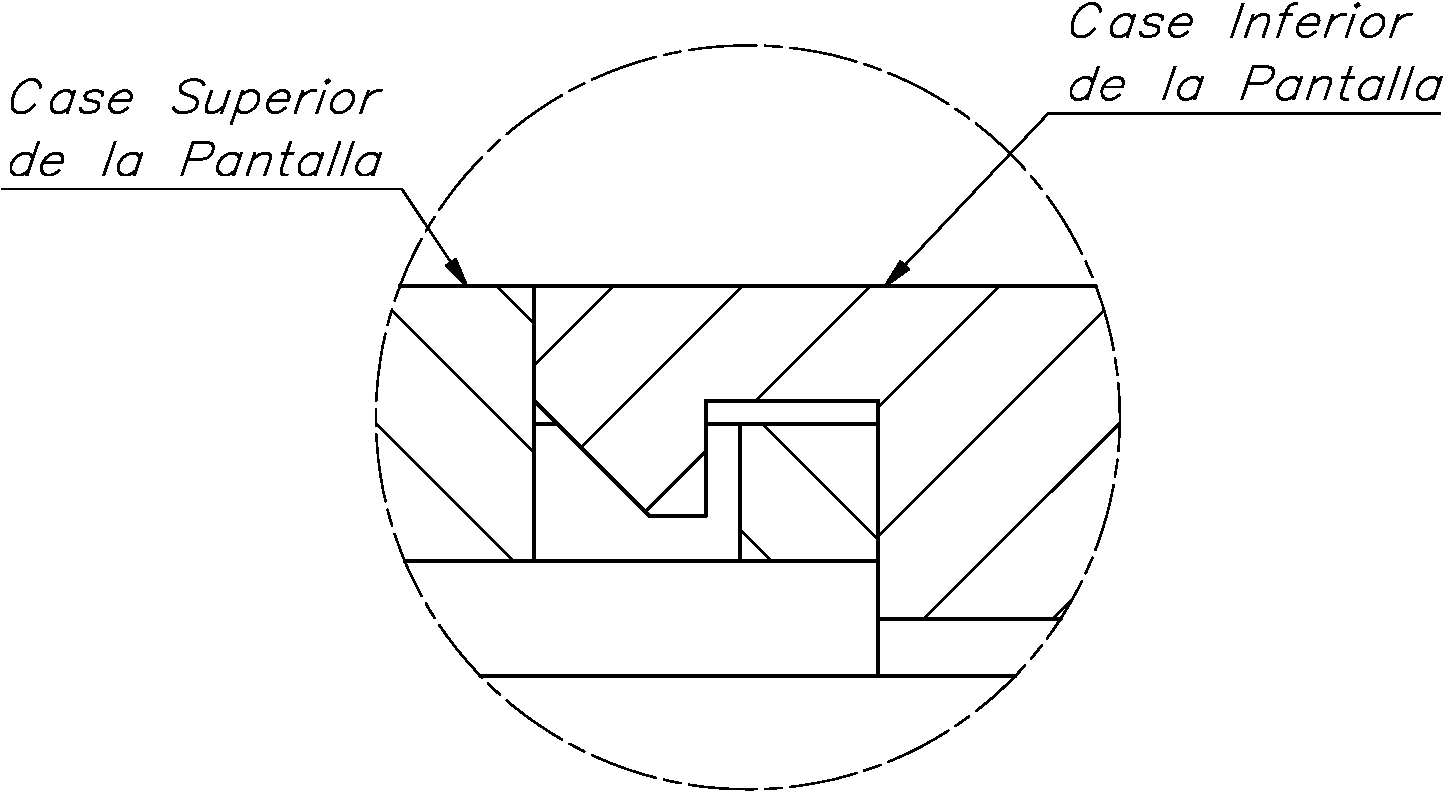
\includegraphics[width=0.9\linewidth]{snap_pantalla.pdf}
  \caption{Snap fit del ensamble del Case de la Pantalla}
  \label{fig:snap_pantalla}
\end{subfigure}
\caption{Detalles del ensamble del case de la pantalla}
\label{fig:test}
\end{figure}


La parte superior del case presiona a la placa electrónica  de la pantalla contra la parte inferior del case usando 4 columnas. Esto se puede observar en la Fig.~\ref{fig:union_pantalla}. Además el snap fit (Fig.~\ref{fig:snap_pantalla}) de este ensamble es distinto del usado en el case principal. En esta ocasión el ángulo de entrada es \SI{45}{\degree} pero el ángulo de salida es \SI{90}{\degree}. Esto significa que la unión es inseparable, ya que el ángulo de entrada permitirá el ensamble y el de salida lo impedirá. Esto se debe a que la pantalla se podrá mover para acomodarse al conductor en cada situación, lo que hace necesario que el case no se separe por error.


\begin{figure}[hbt!]
\centering
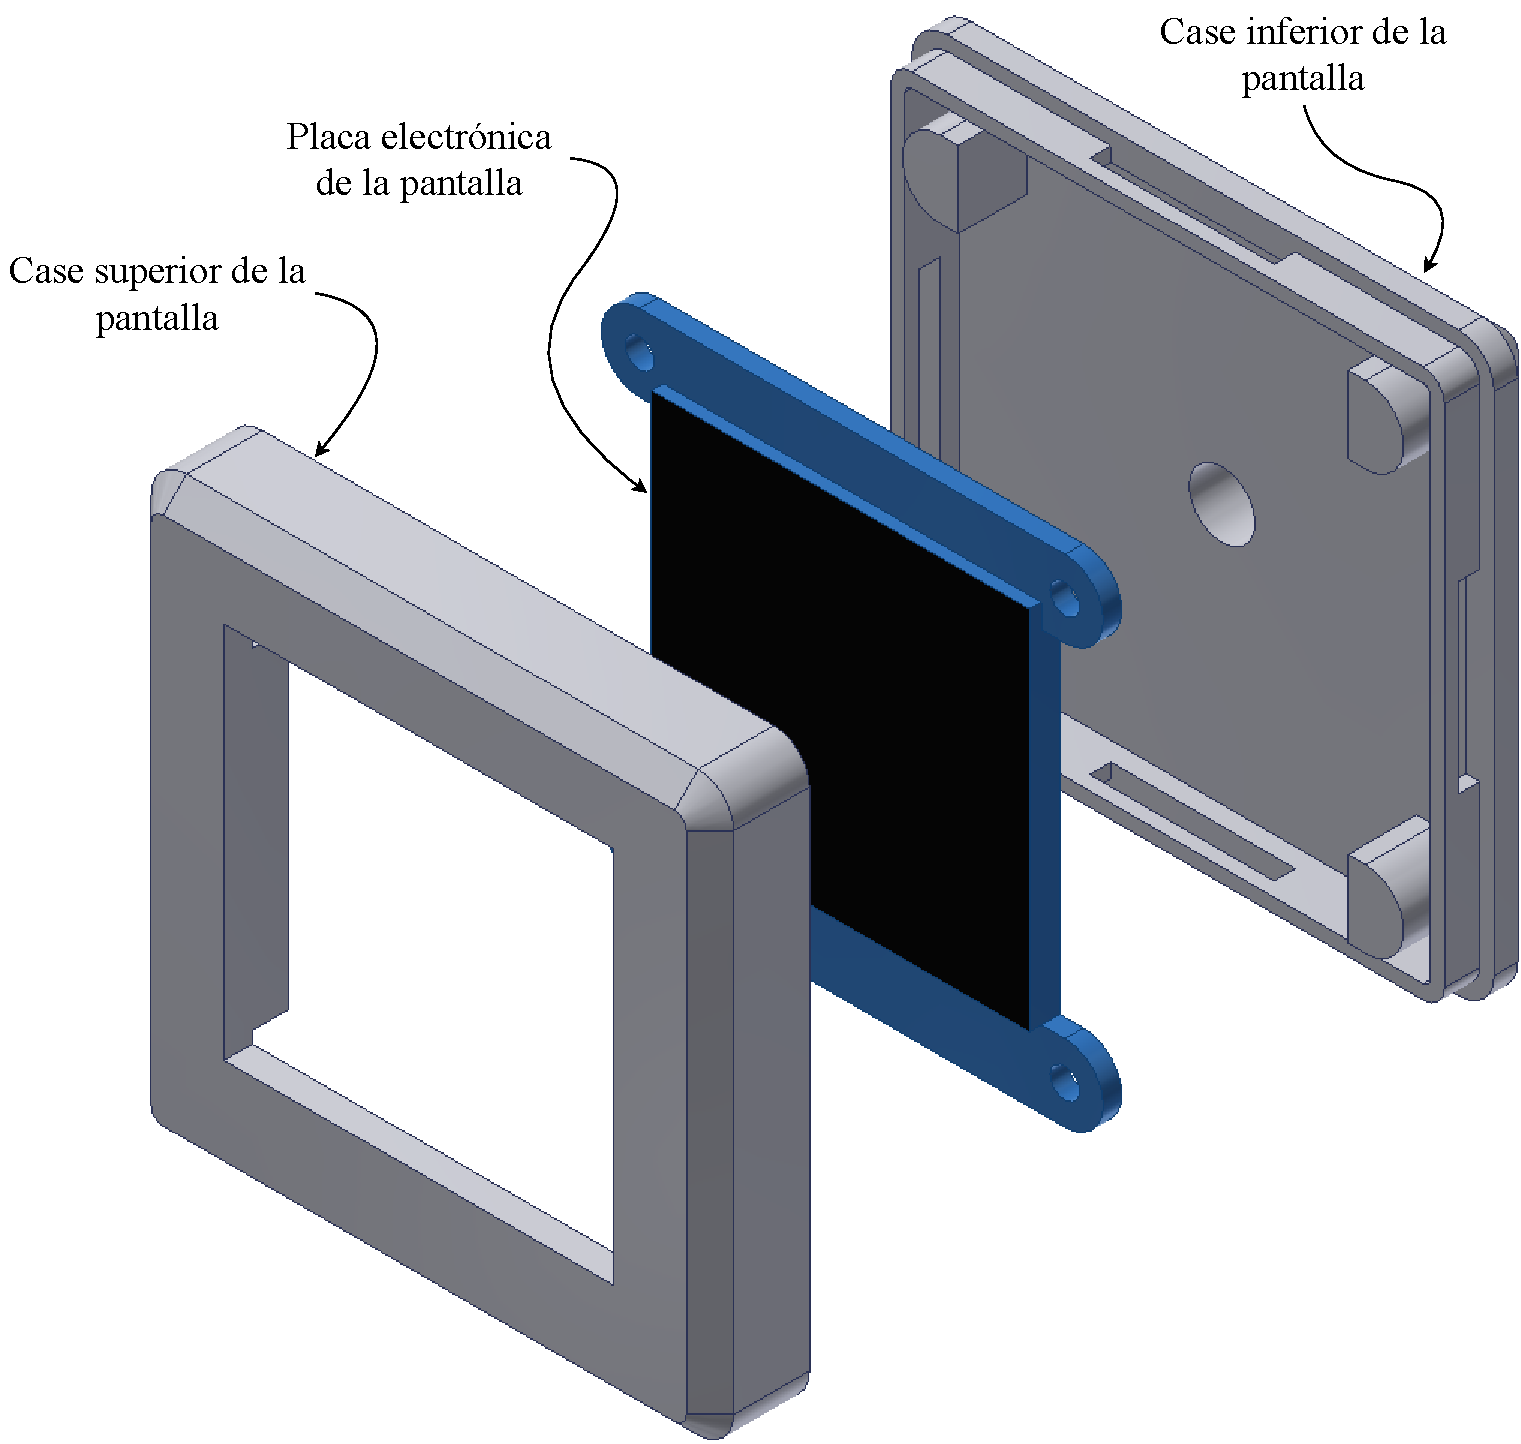
\includegraphics[width=0.8\textwidth]{exploded_2.pdf}
\caption{Vista de explosión del case de la pantalla.}
\label{fig:exploded_pantalla}
\end{figure}

\newpage

\section{Diseño del software de reconocimiento de estilo de conducción}

En esta sección se describe usando diagramas de flujo y pseudocódigo el funcionamiento de la parte de software del sistema de reconocimiento de estilo de conducción. El software consiste en dos partes, la primera se lleva a cabo en cada dispositivo (clientes) y la segunda en un servidor central.

Como se puede observar en la Fig.~\ref{fig:Bloques_software} los clientes envían la información necesaria al servidor central y este clasifica el estilo conducción de cada cliente y los envía de vuelta. Además el servidor mostrará un resumen de los datos recopilados a través de una página web. Los datos mostrados dependen de la persona que inicie sesión en la página. Los conductores podrán ver su puntaje acumulado por día y su historial, y el personal de la empresa podrá ver todos los datos recopilados (Posiciones de los vehículos, consumo, puntaje de los clientes) y resúmenes estadísticos.

\begin{figure}[hbtp!]
\centering
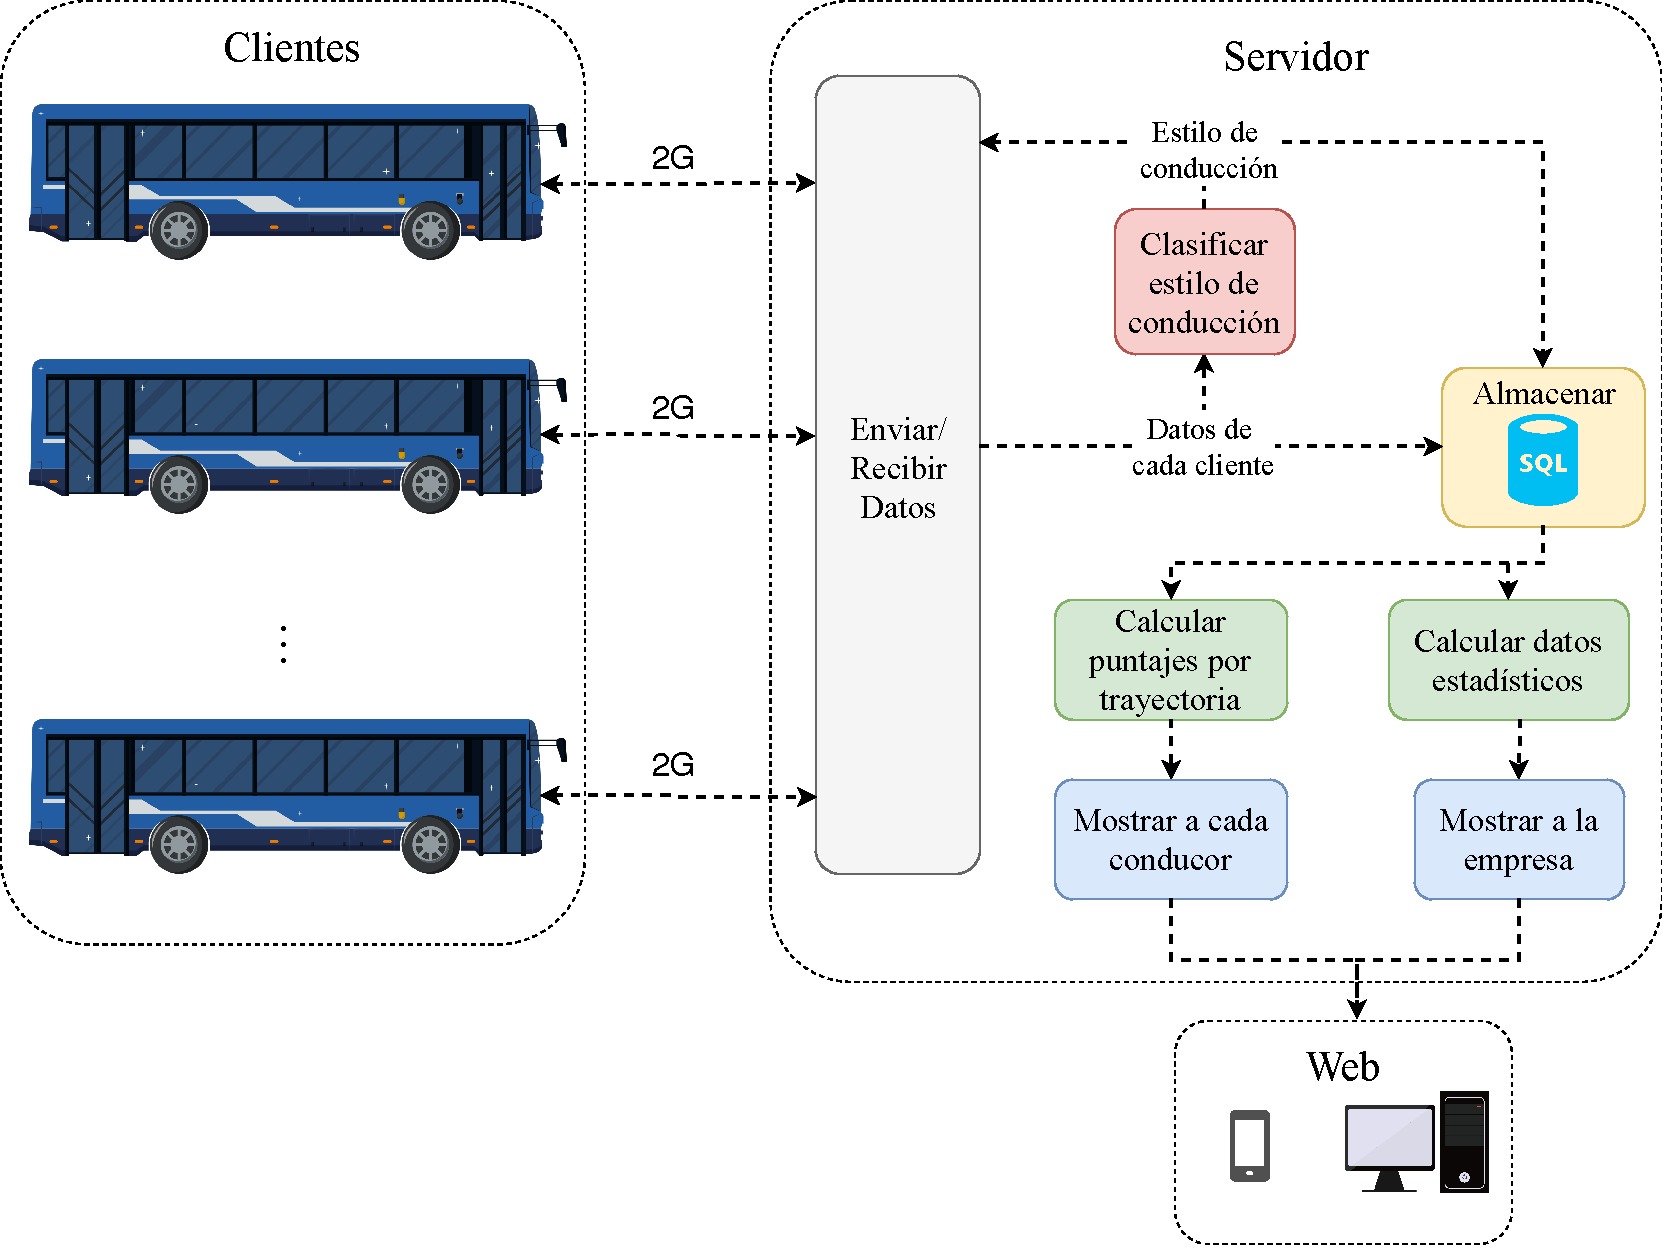
\includegraphics[width=\textwidth]{Bloques_software.pdf}
\caption{Diagrama de bloques del software.}
\label{fig:Bloques_software}
\end{figure}

\subsection{Software de los dispositivos cliente}

Cada dispositivo cliente se coloca en un bus para recopilar datos y enviarlos al servidor. Su funcionamiento se puede apreciar en la Fig.~\ref{fig:Flujo_cliente}. Se inicia el programa al energizar el dispositivo. Luego, este tratará de conectarse al servidor por medio de Internet. Solo al lograr tener una conexión se inicia la recopilación de datos.

El siguiente paso es recopilar los datos de los sensores (IMU, GPS y OBD2). Estos datos necesitan un pre-procesamiento antes de poder ser enviados al servidor. Este pre-procesamiento se lleva a cabo en la función "Sensor Fusion", la cual será explicada más adelante.

A continuación, se almacenan los datos y se repite el proceso durante \SI{1}{s} para luego enviar todos los datos recopilados al servidor. Los datos que se van a enviar se pueden apreciar en la Tabla~\ref{diag:datos_enviar} junto a su tamaño en bytes (Si son representados como texto). Se obtienen estos datos a una frecuencia de \SI{25}{Hz}.

Como se puede apreciar en las Ecuaciones \ref{eq:data_acum1} y \ref{eq:data_acum2}, en \SI{1}{s} de tiempo se acumulan \SI{1625}{bytes}. Estos bytes tardan en enviarse a una velocidad de \SI{85.6}{Kbits/s} a través del módulo 2G solo \SI{0.15}{s}. Luego este ciclo vuelve a repetirse.


\begin{align}
\SI{1625}{bytes}=\SI{65}{bytes}\times\SI{25}{Hz}\times\SI{1}{s} \label{eq:data_acum1} \\
\frac{\SI{1625}{bytes}\times\SI{8}{bits/bytes}}{\SI{85.6}{Kbits/s}}=\SI{0.76}{s}
\label{eq:data_acum2}
\end{align}

\begin{figure}[hbtp!]
\centering
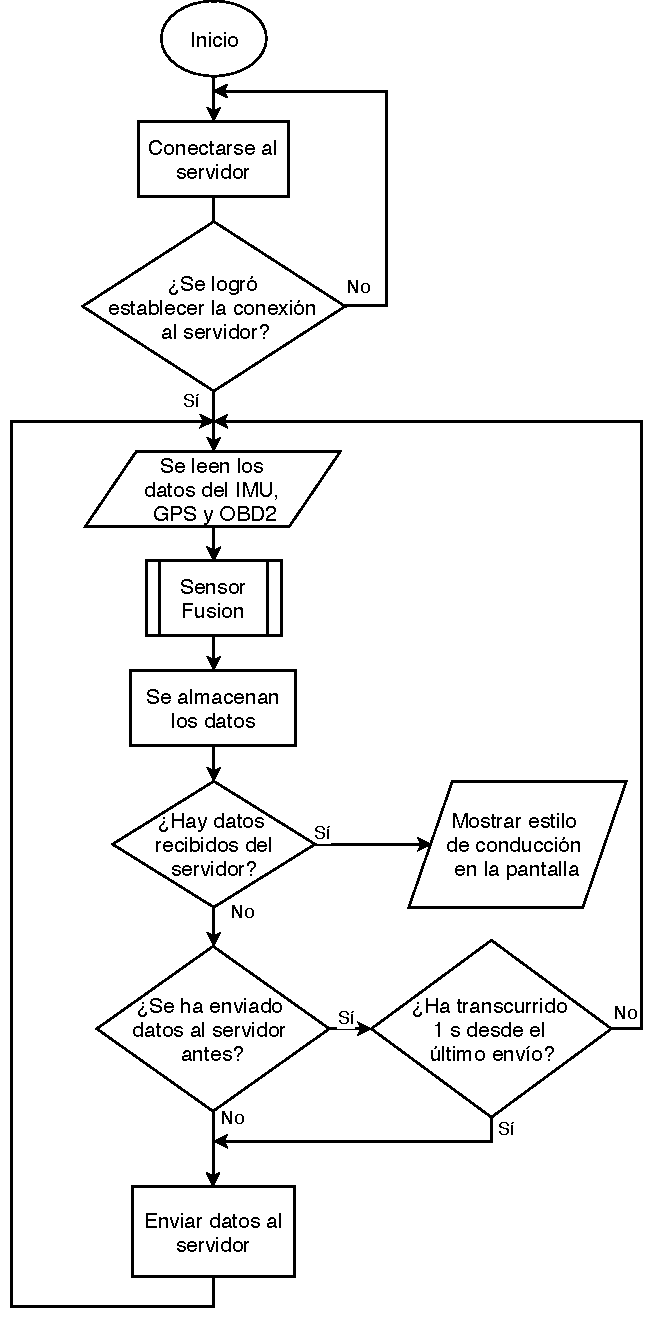
\includegraphics[width=0.7\textwidth]{Flujo_cliente.pdf}
\caption{Diagrama de flujo del software de los dispositivos cliente.}
\label{fig:Flujo_cliente}
\end{figure}

\bgroup
\def\arraystretch{1}%  1 is the default, change whatever you need
\begin{table}[htbp!]
\centering
\caption[Datos a enviar con su tamaño en bytes]{Datos a enviar con su tamaño en bytes.}
\begin{tabular}{ll}
\toprule
Datos & Tamaño en bytes \\ \midrule
Tiempo en ms & 8 \\
Aceleración frontal & 6 \\
Aceleración lateral & 6 \\
Yaw & 6 \\
Latitud & 9 \\
Longitud & 9 \\
Velocidad & 6 \\
RPM & 6 \\
Carácteres separadores & 9 \\ \midrule
Total & 65 \\ \bottomrule
\end{tabular}
\label{diag:datos_enviar}
\end{table}
\egroup

%\subsubsection{Función Sensor Fusion}

\subsection{Software del servidor}

El servidor se encarga de procesar los datos de todos los conductores. Por lo que se tienen varias instancias siendo ejecutadas concurrentemente. Cada instancia esta asociada con un vehículo y conductor. En la Fig.~\ref{fig:Flujo_servidor_principal} se puede observar el proceso que se encarga de administrar las instancias. Luego de crear una instancia para cada vehículo, cuando se cambia de conductor se usa la instancia que ya existía del vehículo usado y se registra el nuevo conductor. Luego se ejecuta la función "Procesar Datos" que se describirá más adelante. Por último, se cierran todas las instancias luego de una hora definida por la empresa.

\begin{figure}[bth!]
\centering
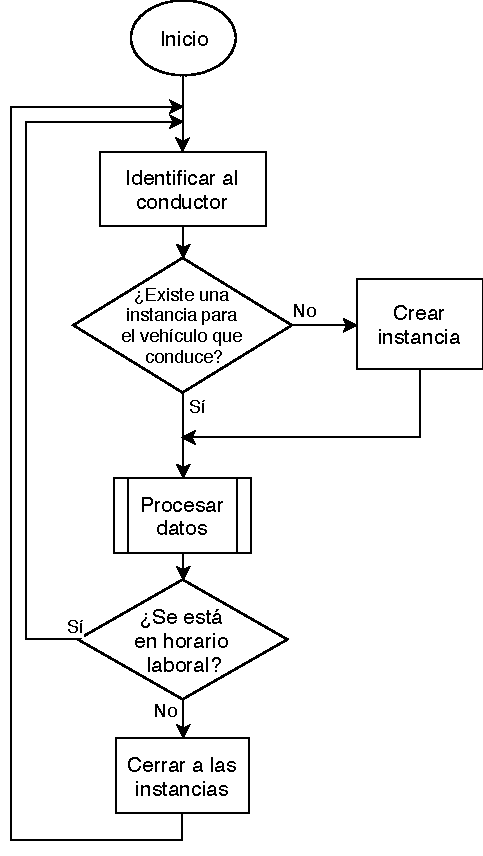
\includegraphics[width=0.55\textwidth]{Flujo_servidor_principal.pdf}
\caption{Diagrama de flujo del software del servidor.}
\label{fig:Flujo_servidor_principal}
\end{figure}

\subsubsection{Función Procesar Datos}
El diagrama de flujo de esta función se puede observar en la Fig.~\ref{fig:Flujo_servidor_procesar}. El primer paso es comprobar si existen nuevos mensajes. Cuando se detecta la presencia de nuevos mensajes se almacenan estos datos y se analizan para detectar el cambio de maniobra.

Cuando se detecta el cambio de maniobra, se ejecuta la función "Clasificar maniobra", que se describirá más adelante. El resultado de esta función es la clasificación del estilo de conducción para la maniobra detectada. Este resultado se almacena y se envía al dispositivo cliente para ser mostrado al conductor.

\begin{figure}[bth!]
\centering
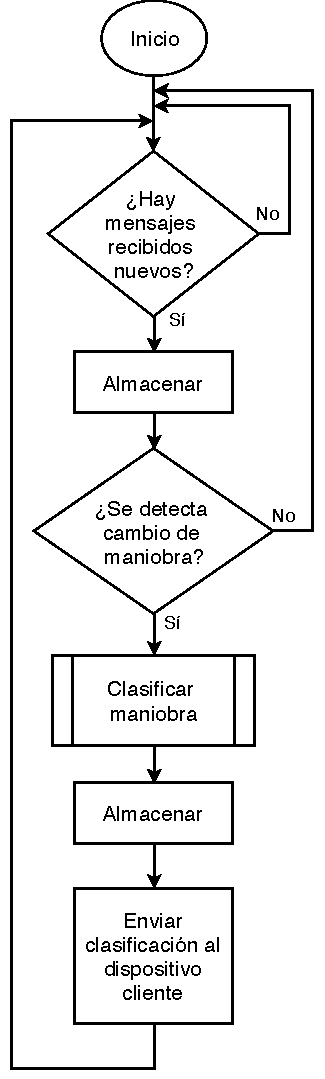
\includegraphics[width=0.3\textwidth]{Flujo_servidor_procesar.pdf}
\caption{Diagrama de flujo de la función Procesar Datos.}
\label{fig:Flujo_servidor_procesar}
\end{figure}

\subsubsection{Función Clasificar maniobra}
Esta función es la encargada de clasificar una maniobra según su estilo de conducción. Como se observa en la Fig.~\ref{fig:Flujo_servidor_clasificar}, el primer paso consiste en extraer todos las muestras de datos que pertenecen a la maniobra. Estos datos van a ser descritos usando características estadísticas para series temporales.

Una vez calculadas estas características, se obtiene por cada maniobra (de varios puntos temporales) una sola instancia . Esta instancia es ahora introducida en el modelo de clasificación que ha sido entrenado previamente. Este modelo nos entregará la clase de estilo de conducción. La etapa del desarrollo del modelo y de su entrenamiento se desarrolla en el Capítulo~\ref{chap:algoritmo}.


\begin{figure}[hbt!]
\centering
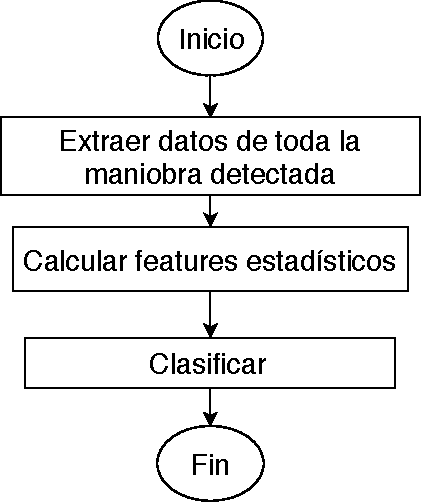
\includegraphics[width=0.4\textwidth]{Flujo_servidor_clasificar.pdf}
\caption{Diagrama de flujo de la función Clasificar maniobra.}
\label{fig:Flujo_servidor_clasificar}
\end{figure}


\subsection{Software de la página web}

La página web permitirá visualizar los datos que estén registrados en la base de datos. Como se ha visto en las secciones anteriores, los datos de cada vehículo y cada conductor con su respectivo puntaje y clasificación para cada maniobra son almacenados en esta base de datos. Esta página web tendrá una etapa de autenticación de usuario, en dónde el usuario iniciará sesión. Existirán dos tipos de usuarios: Conductores y Supervisores. La única diferencia es que los conductores solo podrán acceder a los datos registrados consigo mismo y los supervisores podrán acceder a todos los datos disponibles




















